\documentclass{article}
\usepackage[utf8]{inputenc}

\title{Penalized Regression in the Age of Big Data} %just a filler title, we can change it to whatever we want
\author{Gabriel Ackall$^1$*, Connor Shrader$^2$* \\
		Mentor: Dr. Ty Kim$^3$ \\	
		{\footnotesize $^1$Georgia Tech, Civil and Environmental Engineering} \\
		{\footnotesize $^2$University of Central  Florida, Mathematics} \\
		{\footnotesize $^3$NCA\&T University, Mathematics and Statistics} \\
		{\footnotesize *Authors contributed equally}}
\date{\today}

% Format settings
\setlength{\parskip}{6pt}

% Package imports
\usepackage{fancyhdr}
\usepackage[margin = 1in]{geometry}

\usepackage{amsmath}
\usepackage{amsthm}
\usepackage{listings} % Show code in LaTeX
\usepackage{graphicx} % Figures
\usepackage{caption} % Caption customization
\usepackage{subcaption} % Subfigures
\usepackage{url}
\usepackage{adjustbox}
\usepackage{hyperref} % Clickable ref's

% Caption format
\captionsetup[figure]{font=small}

% Setting up headers and footers
\pagestyle{fancy}
\fancyhead[L]{Penalized Regression}
\fancyhead[R]{Ackall, Shrader}
\fancyfoot[C]{\thepage}

% Set code appearance
\lstset {
	language = R,
	basicstyle = \ttfamily
}

% Clickable link setup
\hypersetup{
	colorlinks=true,
	linkcolor=blue,
	filecolor=magenta,      
	urlcolor=cyan,
	citecolor=blue
}

\newcommand{\argmin}[2]{\underset{#1}{\text{arg min}}\left\{#2\right\}}
\newcommand{\sign}{\text{sign}}
\newcommand{\E}{\text{E}}
\newcommand{\OLS}{\text{OLS}}
\newcommand{\RSS}{\text{RSS}}

\begin{document}
\maketitle

\begin{abstract}
With the prevalence of big data in the modern age, the importance of modeling high dimensional data and selecting influential features has increased greatly. High dimensional data is common in many fields such as genome decoding, rare disease identification, economic modeling, and environmental modeling. However, most traditional regression and classification machine learning models are not designed to handle high dimensional data or conduct variable selection. In this paper, we investigated the use of penalized regression methods instead of, or in conjunction with, the traditional machine learning methods. We focused on lasso, ridge, elastic net, SCAD, MCP, and adaptive versions of lasso, ridge, and elastic net models. For traditional machine learning models, we focused on random forest models, gradient boosting models in the form of XGBoost, and support vector machines. These models were evaluated using factorial design methods for Monte Carlo simulations under various data environments. Tests were conducted for 270 environments, with factors being the number of predictors, number of samples, signal to noise ratio, covariance matrix, and correlation strength. This served to identify the strengths and weaknesses of different penalization techniques in different environments. We also compared different models using empirical datasets to test their viability in real-world scenarios. Additionally, we considered penalization methods outlined earlier in logistic regression models for classifying data. These results were compared to random forest, gradient boosting, and support vector machine classification models using both Monte Carlo data generation methods and empirical data. For regression, we evaluated the models using the test mean squared error and variable selection accuracy; for classification, we considered test prediction accuracy and variable selection accuracy. We found that for both regression and classification, penalized regression models outperformed more traditional machine learning algorithms in most high-dimensional situations or in situations with a low number of data observations. By comparing traditional machine learning methods with penalized regression, we hope to expand the scope of machine learning methods for big data to include the various penalized regression techniques we tested. Additionally, we hope to create a greater understanding of the strengths and weaknesses of each model type and provide a reference for other researchers on which machine learning techniques they should use, depending on a range of factors. \\

\textit{Keywords:} penalized regression, variable selection, classification, machine learning, large $p$ little $n$ problem, Monte Carlo simulations
\end{abstract}

%%%%%%%%%%%%%%%%%%%%%%%%%%%%%%%%%%%%%%%%%%%%%%%%%%%%%%%%%%%%%%%%%%%%%
\section{Introduction}
% introduce readers to our topic and necessary info to better understand the paper

[Better intro paragraph]

Typically, data sets are represented as a table of values. Most columns represent \textbf{predictors} (also called variables, attributes, or features), while the rows represent \textbf{observations} (also called instances). The value in the $i$-th row and $j$-th column represents the value for predictor $j$ in observation $i$. At least one column is designated as a \textbf{response}, which is assumed to be related to some of the predictors in some way. Machine learning models attempt to predict the value of this response from the values of the predictors.

Let $n$ be the number of observations for a data set, and let $p$ be the number of predictors. In most situations, the number of observations greatly exceeds the number of predictors. However, as data collection becomes easier and as statistical modeling techniques are introduced to new disciplines, situations can arise where there are more predictors than observations. For instance, in the field of genomics, there may be thousands of genes that could cause a disease and only a few samples to train from.

In situations where there are more predictors than observations, many traditional machine learning techniques fail to give good predictions. The large number of predictors makes it easy for such models to \textbf{overfit}, meaning that the models make good predictors from the data used to train the model, but perform badly when given new data. 

To resolve this ``large $p$, little $n$'' problem, many algorithms have been introduced to address situations where there are more predictors than observations. Many, but not all, of these techniques use \textbf{variable selection}, meaning that they select the predictors that are most correlated with the response. By ignoring predictors that are not strongly related to the response, the negative consequences of overfitting can be greatly reduced.

This paper investigates various methods used to handle the large $p$, small $n$ problem. We considered subset selection methods such as forward selection, backward selection, stepwise forward selection and stepwise backward selection. In addition, we studied penalized regression models such as ridge regression, LASSO, elastic-net, adaptive LASSO, SCAD, and MCP. Models were trained and evaluated using both Monte Carlo simulations and empirical genomic data.

\subsection{Background}
% We can talk about the necessary background information
% what is linear regression?



Suppose that we have $p$ predictor variables $X_1, X_2, \dotsc, X_p$ and one response variable $Y$ that depends on some (or all) of the predictors. We assume that $Y$ can be expressed as
\begin{equation}\label{eqn:relationship}
	Y = f(X_1, X_2, \dotsc, X_p) + \epsilon
\end{equation}
where $f$ is a function and $\epsilon$ is an independent random error with mean zero. The goal of supervised modeling is to find a function $\hat{f}$ that is a suitable approximation for $f$. To find $\hat{f}$, we use a \textbf{training set}, a set of observations where the response variable $Y$ is already known. Then, using the fitted model, we can predict the value of the response variable $\hat{Y}$ for new observations, even if $Y$ is unknown. Model performance can be evaluated using a \textbf{test set}, which is a set of observations that were not used to train the model.

There are two broad types of supervised models. \textbf{Regression modeling} is used when the response variable $Y$ takes numerical values on a continuous interval. For example, a model that predicts the value of a home is a regression model. On the other hand, if $Y$ can only take discrete values, then \textbf{classification modeling} is used. For instance, a model used to predict whether or not a patient has a disease is classification problem. This paper focuses on regression modeling.

\subsection{Linear Regression and Ordinary Least Squares}

In practice, the function $f$ that relates the predictors to the response is complex. Most statistical models assume that $f$ takes some particular form and estimates a function $\hat{f}$ of that form. For example, many regression models assume that $f$ is a linear function of the predictors; that is, linear models assume that
\begin{equation}\label{eqn:linear-model}
	f(X_1, X_2, \dotsc, X_p) = \beta_0 + \beta_1 X_1 + \beta_2 X_2 + \cdots + \beta_p X_p
\end{equation}
where $\beta_0, \beta_1, \beta_2, \dotsc, \beta_p$ are coefficients. Notice that the coefficient $\beta_0$ is not multiplied with any predictor; it represents an intercept value. Fitting a linear model will give estimates for these coefficient values.

The most common method to approximate the coefficients in a linear model is by \textbf{ordinary least squares}. Suppose that we have $n$ observations in our training set. Let $x_{ij}$ represent the value of predictor $j$ for observation $i$, and let $y_i$ be the response for observation $i$. For some coefficient estimates $\beta_0, \beta_1, \beta_2, \dotsc, \beta_p$, the expression
\begin{equation}
	y_i - (\beta_0 + \beta_1 x_{i1} + \beta_2 x_{i2} + \cdots + \beta_p x_{ip})
\end{equation}
is called the \textbf{residual} for observation $i$; it is the difference between the true response value and the predicted response variable using the given coefficient values. Ordinary least squares chooses the coefficients $\beta_0, \beta_1, \beta_2, \dotsc, \beta_p$ that minimize the \textbf{residual sum of squares}
\begin{equation}\label{eqn:RSS}
	\text{RSS} = \sum\limits_{i = 1}^n (y_i - (\beta_0 + \beta_1 x_{i1} + \beta_2 x_{i2} + \cdots + \beta_p x_{ip}))^2
\end{equation}
Intuitively, if the residual sum of squares is low, then the differences between the response variable and its estimates is low. Thus, by minimizing the residual sum of squares, the function obtained from ordinary least squares is a relatively good approximation for $f$. Figure \ref{fig:ols} demonstrates a model fitted with ordinary least squares when there is a single predictor variable.

\begin{figure}[!h]
	\centering
	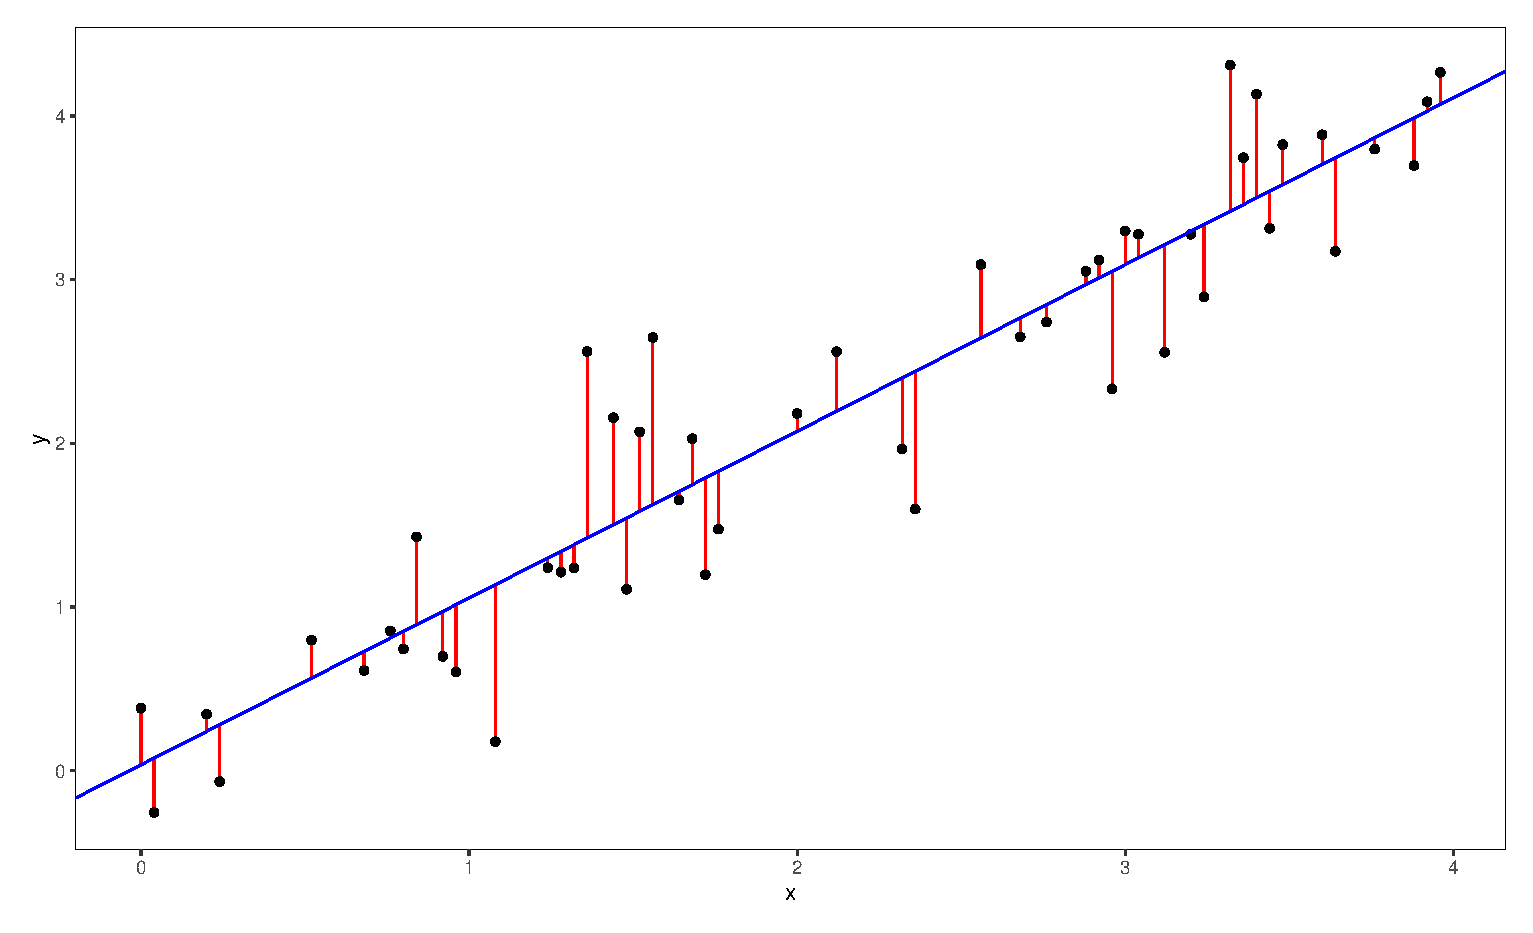
\includegraphics[width = 4in]{images/ols.eps}
	\captionsetup{width=4in}
	\caption{Ordinary least squares fitting with one predictor using simulated data. The blue line represents the line found by ordinary least squares, and the red line segments are the residuals.}
	\label{fig:ols}
\end{figure}

One reason that ordinary least squares is popular is because it is very easy to compute. Let $\beta = [\beta_0, \beta_1, \beta_2, \dotsc, \beta_p]^\top$ be a $(p + 1) \times 1$ vector of coefficient values and let $\mathbf{X}$ be a $n\times (p + 1)$ matrix where each row contains the predictor values for one observation, with an additional value of 1 in the first entry (this extra value corresponds to the intercept coefficient $\beta_0$, which is not truly a predictor). Then $\mathbf{X}\beta$ is a vector of the estimated response values for our choice of $\beta$. Let $\mathbf{y}$ represent the true response values. Then $\mathbf{y} - \mathbf{X}\beta$ is a vector of residuals. To choose coefficient estimates that minimize the residual sum of squares, we compute
\begin{equation}
	\hat{\beta}^{\text{OLS}} = \argmin{\beta}{(\mathbf{y} - \mathbf{X}\beta)^\top (\mathbf{y} - \mathbf{X}\beta)}
\end{equation}
where $(\mathbf{y} - \mathbf{X}\beta)^\top (\mathbf{y} - \mathbf{X}\beta)$ is the same residual sum of squares seen in Equation \ref{eqn:RSS}. From \cite{friedman2001elements}, this gives us the solution
\begin{equation}\label{eqn:ols-solution}
	\hat{\beta}^{\text{OLS}} = (\mathbf{X}^\top \mathbf{X})^{-1} \mathbf{X}^\top \mathbf{y}
\end{equation}

Another advantage of ordinary least squares is that it is an unbiased linear model. This means that if the relationship between the response variable and the predictors is actually linear (as given in Equation \ref{eqn:linear-model}), then the expected value of the coefficient vector $\hat{\beta}^\text{OLS}$ is equal to the actual coefficient vector $\beta$. Furthermore, the \textbf{Gauss-Markov theorem} states that if the random error $\epsilon$ is independent and has constant variance, then ordinary least squares has the lowest variance among all linear unbiased estimators. In other words, the coefficient estimates given by ordinary least squares are relatively close to the actual coefficient values when compared to other unbiased linear estimators. This makes ordinary least squares a relatively consistent model.

If ordinary least squares is unbiased and has the lowest variance among all unbiased models, why should we use any other type of linear model? Despite having a lower variance than other unbiased models, ordinary least squares can still have a high variance. This is especially an issue when the number of predictors $p$ is large compared to the number of observations $n$. As $p$ gets closer to $n$, a model fitted with ordinary least squares will typically \textbf{overfit} to the training set. This means that the fitted model makes very good predictions with the training data, but performs poorly when given test data that wasn't used to fit the model. Overfitting occurs because of the random error from Equation \ref{eqn:relationship}. Ordinary least squares is unable to distinguish between signal and noise, so it will tend to assume predictors are more strongly related to the response than they actually are.

In the extreme case where $p$ exceeds $n$, the matrix $\mathbf{X}^\top \mathbf{X}$ from Equation \ref{eqn:ols-solution} becomes non-invertible. This means that there are many coefficient estimates that minimize the residual sum of squares. In fact, any of these coefficient estimates creates a perfect fit to the training data, which will result in very bad predictions with test data.

By using models that have a small amount of bias, the high variance of ordinary least squares can be mitigated. Liu et. al. in \cite{liu2020logsum} describe three types of variable selection algorithms. \textbf{Filter methods} work by evaluating the ability for each individual predictors to predict the response; then, a model is fit using the predictors selected. \textbf{Wrapper methods} fit models using different subsets of predictors and choose the model that has the best performance. Finally, \textbf{embedded methods} perform variable selection during the model training process. This paper focuses on wrapper methods and embedded methods. In addition, we also used several non-linear machine learning methods to draw a comparison between linear regression models and non-linear models.

\subsection{Subset Selection Methods}
% We can review some relevant literature such as Tibshrani et. al. lasso methods, ridge regression, enet, SCAD, or whatever else we want to do.

\textbf{Subset selection methods} are wrapper methods that attempt to find a subset of the predictors $X_1, X_2, \dotsc, X_p$ that are most correlated with the response variable $Y$. These algorithms usually fit models for many different subsets and choose the subset of predictors that results in the best model. Although subset selection techniques can be applied to many types of models, we will focus on subset selection with linear regression.

There are two main benefits to using subset selection methods. By reducing the set of available predictors to just those that are strongly related to the response, overfitting can be mitigated by ignoring predictors that provide little improvement to model performance. Another benefit of subset selection is that it creates a more interpretable model. If a data set includes thousands of predictors but only a few are related to the response, a model found using subset selection will be easier to understand than a model that relies on all of the parameters. 

\textbf{Best subset selection} is a subset selection method that considers every possible combination of predictors. For every possible value of $k$ between 0 and $p$, best subset selection will fit the ${p\choose k}$ possible models using $k$ predictors. Then, the best model for each value of $k$ is chosen based on some performance metric. Finally, a final model can be selected from the $(p + 1)$ remaining models, ranging from an empty model with no predictors to a full model with all of the predictors. If $p$ is larger than $n$, then models are only fit for subsets with $n$ or less predictors since ordinary least squares cannot be used when there are more predictors than observations.

Although best subset selection is guaranteed to find the subset of predictors that optimize the chosen metric, this method is computationally expensive. For a data set with $p$ predictors, $2^p$ possible combinations must be considered. This makes best subset selection infeasible when the number of predictors is too large.

Two alternative methods to best subset selection are \textbf{forward selection} and \textbf{backward selection}. Forward selection begins by fitting a model with no predictors (only the intercept is non-zero) and iteratively adds predictors into the model. The predictor added at each step is chosen to best increase the model fit. Conversely, backward selection starts from the full (ordinary least squares) model with all $p$ predictors and repeatedly removes predictors. Then, like best subset selection, the final model is chosen from the candidate models fitted at each step. Note that backward selection can only be used when $p\leq n$ since ordinary least squares cannot be used when $p>n$. Forward selection can always be used.

Although forward and backward selection will not always encounter the best possible model, these methods avoid the exponential runtime of best subset selection. Consequently, forward and backward selection can be used for larger values of $p$.

The models produced by forward and backward selection can be improved by allowing predictors to be added and removed in the same algorithm. \textbf{Forward stepwise selection} begins with an empty model and iteratively improves the model by either adding a new predictor or removing an obsolete one. \textbf{Backward stepwise selection} works in the same way but starts with the full model. Like backward selection, backward stepwise selection can only be used when $p\geq n$. These techniques take longer to run than ordinary forward and backward selection, but they are more likely to find the best possible model.

When fitting a model using any of the subset selection methods, the performance metric used when selecting the best model is very important. At first, it may seem reasonable to choose a metric such as the residual sum of squares from Equation \ref{eqn:RSS}. However, many metrics, including the residual sum of squares, only describe a model's performance on training data. This is problematic because including more predictors will always decrease the residual sum of squares on the training data. If $p\leq n$, then the model fitted with all $p$ predictors is exactly the same model produced by ordinary least squares, which by definition minimizes the residual sum of squares! If $p>n$, then a model with the maximum possible number of predictors would be selected.

If we wish to produce a model that makes reliable predictions on test data, we must use a different performance metric. Two of the most common metrics used for this purpose are the \textbf{Akaike Information Criterion} (AIC) and the \textbf{Bayesian Information Criterion} (BIC). These metrics can be expressed in terms of the log-likelihood function. In the special cases where we have a linear model where the random error $\epsilon$ is Gaussian, the Akaike Information Criterion can instead be expressed as
\begin{equation}
	\text{AIC} = \frac{1}{n\hat{\sigma}^2}(\RSS + 2p\hat{\sigma}^2)
\end{equation}
up to a constant, where $\hat{\sigma}^2$ is the estimated value of the variance of $\epsilon$ and RSS is the residual sum of squares from Equation \ref{eqn:RSS} \cite{james2017islr}. The Bayesian Information Criterion is
\begin{equation}
	\text{BIC} = \frac{1}{n\hat{\sigma}^2}(\RSS + \ln(n)p\hat{\sigma}^2)
\end{equation}
up to a constant. These metrics work by using the residual sum of squares plus some additional penalty that increases when $p$ is large. As a result, models that minimize AIC or BIC will have fewer predictors than models chosen just by minimizing the residual sum of squares. This can result in a model that has both a good training error and test error. If $n>7$, then $\ln(n)>2$ and so the penalty for BIC is larger than the penalty for AIC. Hence, a model selected using BIC will typically have fewer parameters than a model selected by AIC.

In addition to AIC and BIC, there are several other metrics that modify training error to estimate test error, such as $C_p$ and adjusted $R^2$ \cite{james2017islr}. However, this paper will focus on AIC and BIC.
\subsection{Penalized Regression}

In general, \textbf{penalized regression} works by fitting a model that punishes large coefficient estimates. By forcing coefficient values to shrink, the resulting model will have relatively low variance. Most, but not all, of these methods can perform variable selection. For the remainder of this section, let $\beta$ represent a single arbitrary coefficient value, rather than a vector of coefficient values.

All of the penalized regression methods in this paper solve an optimization problem of the form
\begin{equation}\label{eqn:penalized-regression-lambda}
	\hat{\beta}=\argmin{\beta}{\sum\limits_{i = 1}^N(y_i - (\beta_0 + \beta_1 x_{i1} + \beta_2 x_{i2} + \cdots + \beta_p x_{ip})) + \lambda\sum\limits_{j = 1}^p P(\beta_j)}
\end{equation}
where the first summation is the usual residual sum of squares, $\lambda\geq 0$ is a hyperparameter that controls the strength of the penalty, and $P(\beta)$ is a penalty function applied to each of the coefficients (but not the intercept term). In general, $P(\beta)$ is an even function that is non-decreasing as $\vert \beta \vert$ increases. If $\lambda = 0$, then we have the usual ordinary least squares estimator. As $\lambda$ increases, a stronger penalty is applied which will decrease the coefficient values. As $\lambda$ approaches $\infty$, the model becomes an empty model where only the intercept term is non-zero.

A similar way to express penalized regression is with the form
\begin{equation}\label{eqn:penalized-regression-t}
	\hat{\beta} = \argmin{\beta}{\sum\limits_{i = 1}^N(y_i - (\beta_0 + \beta_1 x_{i1} + \beta_2 x_{i2} + \cdots + \beta_p x_{ip}))} \quad \text{subject to} \quad \sum\limits_{j = 1}^p P(\beta_j)\leq t
\end{equation}
where $t$ is a hyperparameter. In this form, penalized regression fits the ordinary least squares such that the sum of the penalties of the coefficients are kept below some threshold. It can be shown that for every value of $\lambda$ from Equation \ref{eqn:penalized-regression-lambda}, there is a value of $t$ from \ref{eqn:penalized-regression-t} that gives equivalent coefficient estimates \cite{james2017islr}. Most algorithms to fit penalized regression models use the form given in Equation \ref{eqn:penalized-regression-lambda}, but the form in Equation \ref{eqn:penalized-regression-t} may be considered more intuitive.

When fitting penalized regression models, the choice of $\lambda$ is very important. If $\lambda$ is too small, then models may be overfit just like ordinary least squares; on the other hand, if $\lambda$ is large, then the resulting models are highly biased and the resulting models may be underfit. In practice, the best value of $\lambda$ can be selected using \textbf{cross-validation}. This process involves splitting the training set into $k$ disjoint subsets of equal size called \textbf{folds}. Then, $k$ models are fitted for different values of $\lambda$, where one fold is used as a testing set and the other $(k - 1)$ folds are used for training. The value of $\lambda$ that results in the lowest test error can then be selected.

\textbf{Ridge regression} is a penalized regression model that uses the penalty function $P(\beta) = \beta^2$ \cite{hoerl1970ridge}. One advantage of ridge regression is that it can handle highly correlated data better than ordinary least squares. When predictors are correlated with each other, some algorithms have a hard time distinguishing which predictors are actually related to the response. One other benefit of ridge regression is that it can be used when $p>n$.

One drawback of ridge regression is that it cannot perform variable selection. It can shrink coefficients towards zero, but it cannot set coefficients to be exactly zero.

The \textbf{least absolute shrinkage and selection operation} (LASSO) is a shrinkage method with a very similar form to ridge regression \cite{tibshirani1996regression, james2017islr, james2013introduction}. The penalty function for LASSO is $P(\beta) = \vert \beta \vert$.

Unlike ridge regression, LASSO regression can perform variable selection by setting coefficients to zero. This makes LASSO regression favorable when most predictors are not related to the response variable. On the other hand, if the response truly does depend on all of the predictors, then LASSO regression may incorrectly set some coefficients to zero. In addition, LASSO regression does not have a closed-form solution, but computing the coefficients is still efficient.

Figure \ref{fig:ridge-lasso-diagram} provides a visual explanation for why ridge regression cannot perform variable selection while LASSO regression can. Suppose that there are $p = 2$ predictors. The red circle in Figure \ref{fig:ridge-diagram} represents the circle $\beta_1^2 + \beta_2^2 \leq 1$, which is the penalty boundary for ridge regression in the form given in Equation \ref{eqn:penalized-regression-t} when $t = 1$. The red square in Figure \ref{fig:lasso-diagram} represents the boundary $\vert \beta_1 \vert + \vert \beta_2 \vert \leq 1$ for LASSO regression. The point in the center of the blue ellipses represents the values of $\beta_1$ and $\beta_2$ that ordinary least squares would produce. Because this point is not within either of the red regions, ridge regression and LASSO regression will give different coefficient estimates. The blue ellipses around this point represent contour curves for the residual sum of squares function, which is a quadratic function of $\beta_1$ and $\beta_2$. The first interception of these ellipses with the red regions represents the coefficient values selected by ridge and LASSO regression, since it represents the point within the red region with the lowest residual sum of squares. Because of the round boundary for ridge regression, the intersection in Figure \ref{fig:ridge-diagram} occurs when $\beta_1$ and $\beta_2$ are both positive. For LASSO regression in Figure \ref{fig:lasso-diagram}, the intersection occurs at a corner where $\beta_1=0$. Thus, LASSO regression has set $\beta_1$ to zero, while $\beta_1$ is non-zero for ridge regression.

\begin{figure}[!h]
	\centering
	\begin{subfigure}[b]{0.45\textwidth}
		\caption{RSS contours and the ridge penalty boundary.}
		\label{fig:ridge-diagram}
		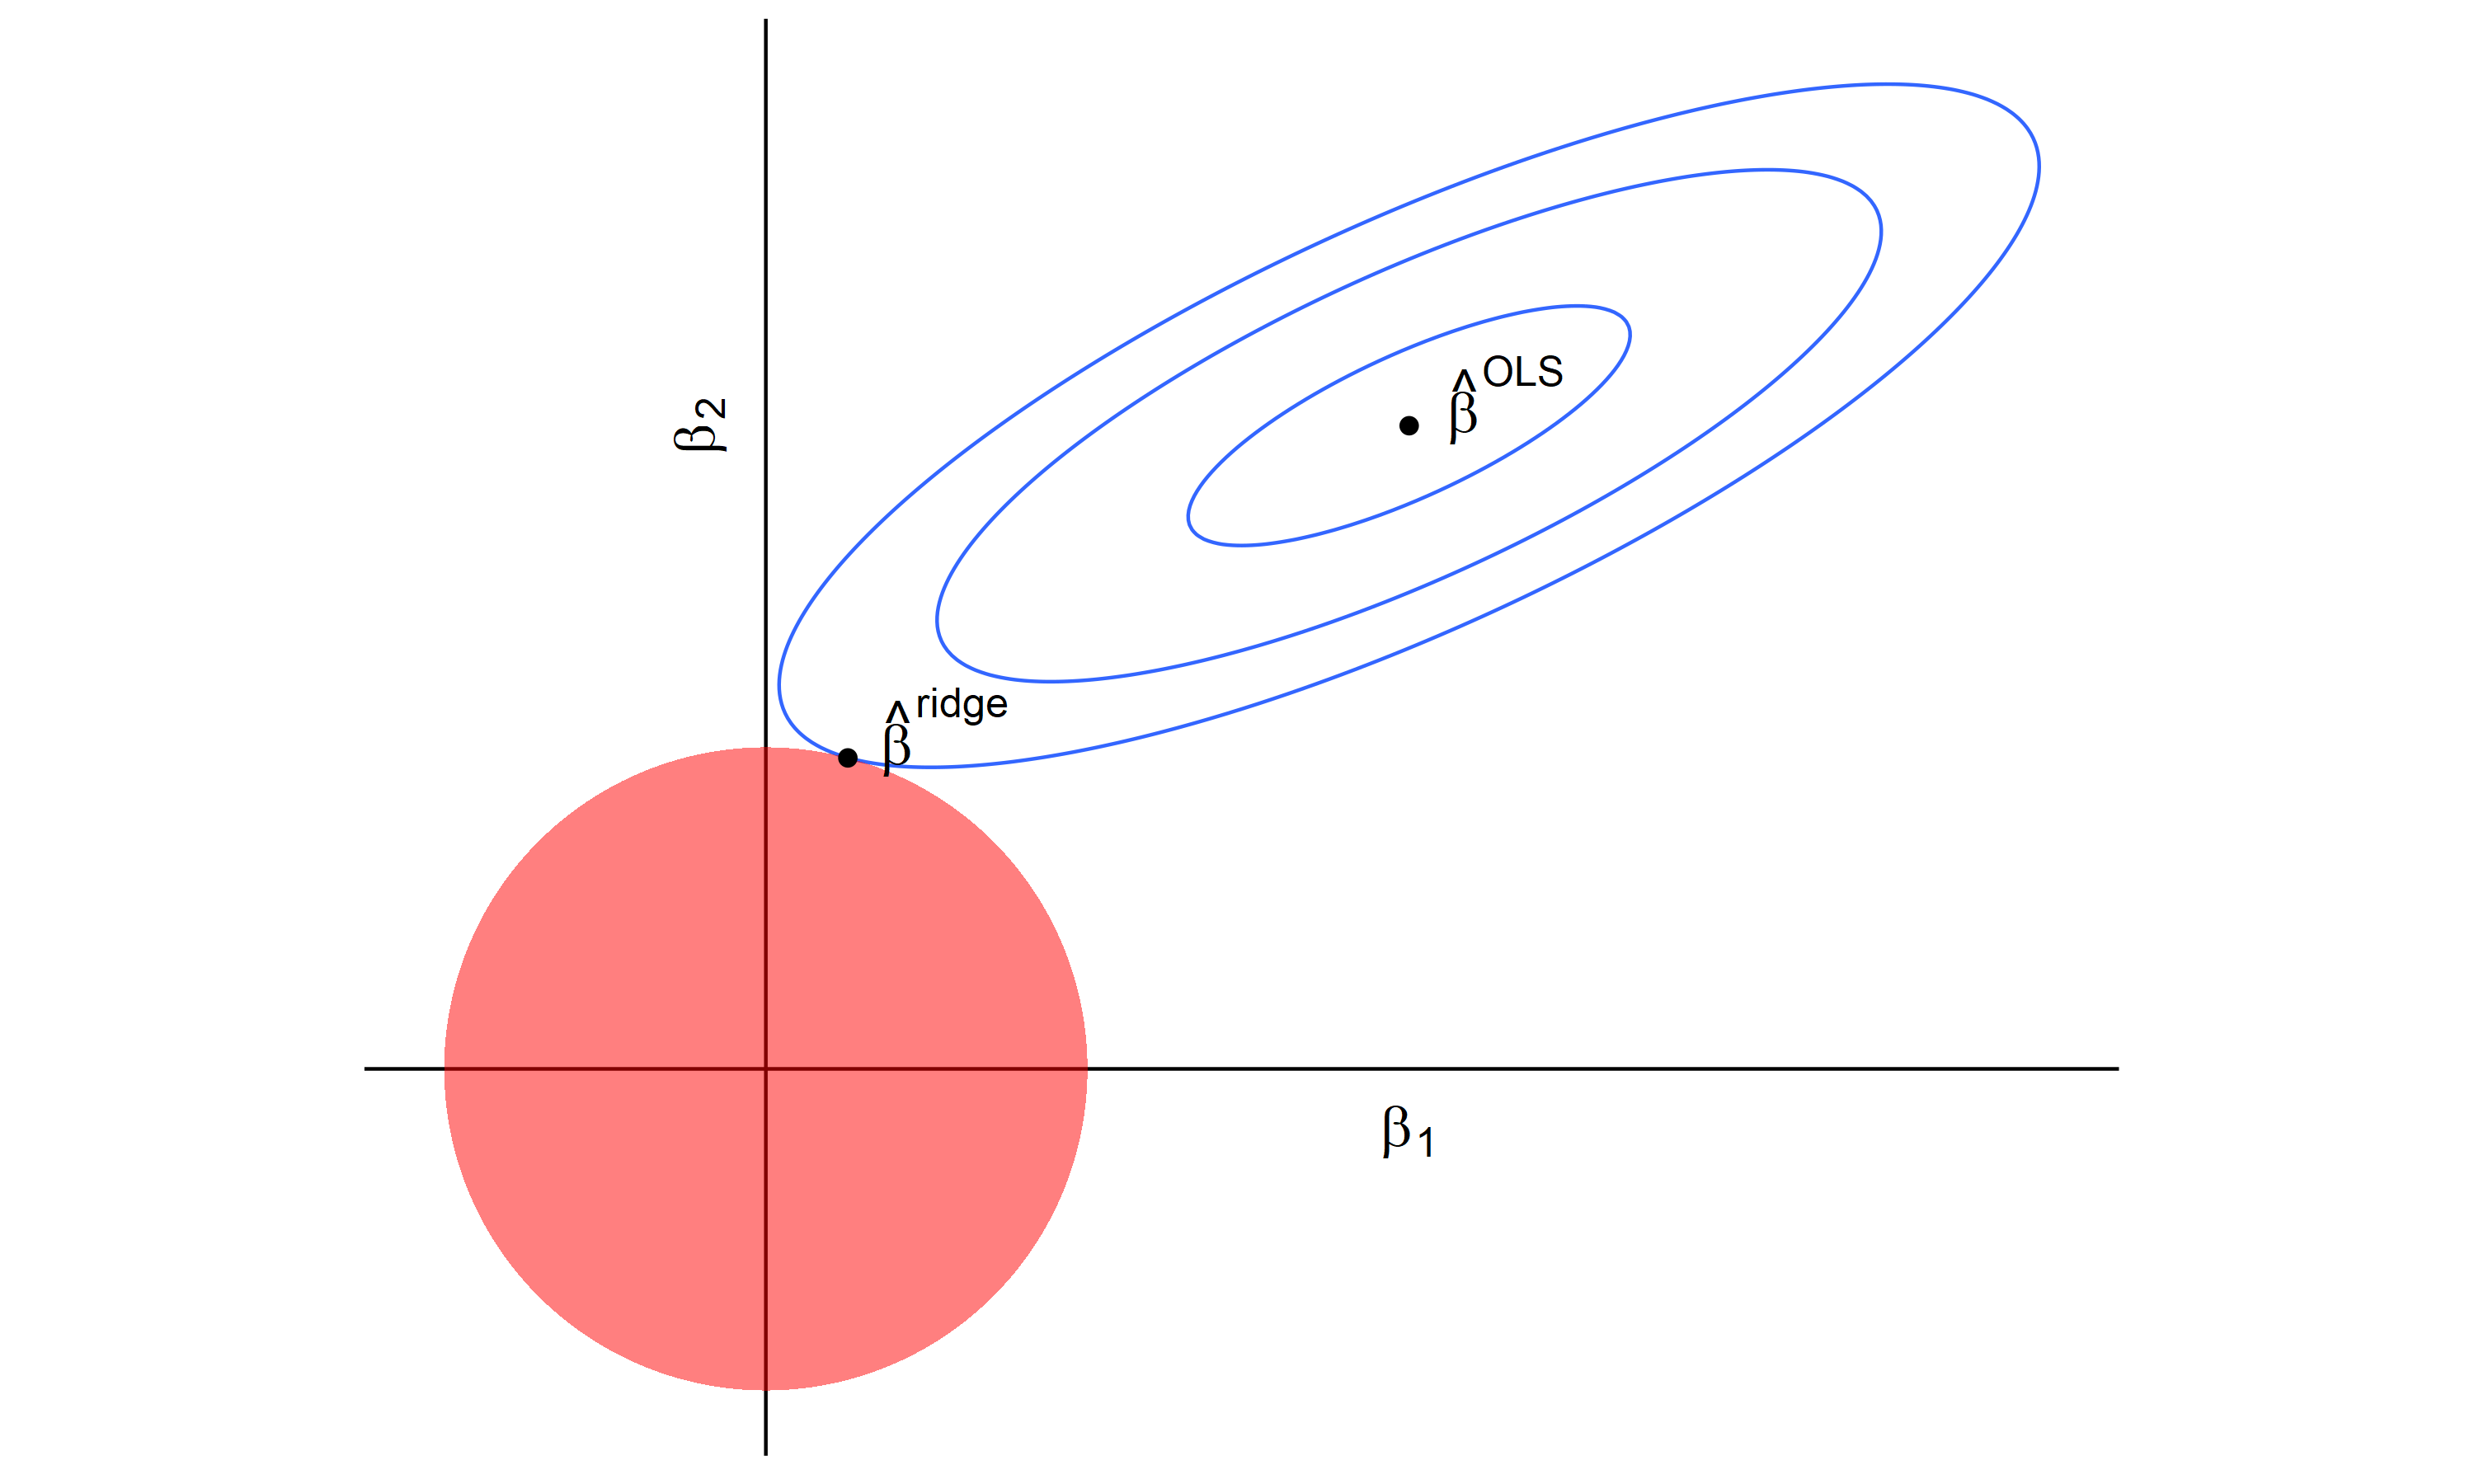
\includegraphics[width=\textwidth]{images/ridge-diagram.png}
	\end{subfigure}
	\hspace{30pt}
	\begin{subfigure}[b]{0.45\textwidth}
		\caption{RSS contours and the lasso penalty boundary.}
		\label{fig:lasso-diagram}
		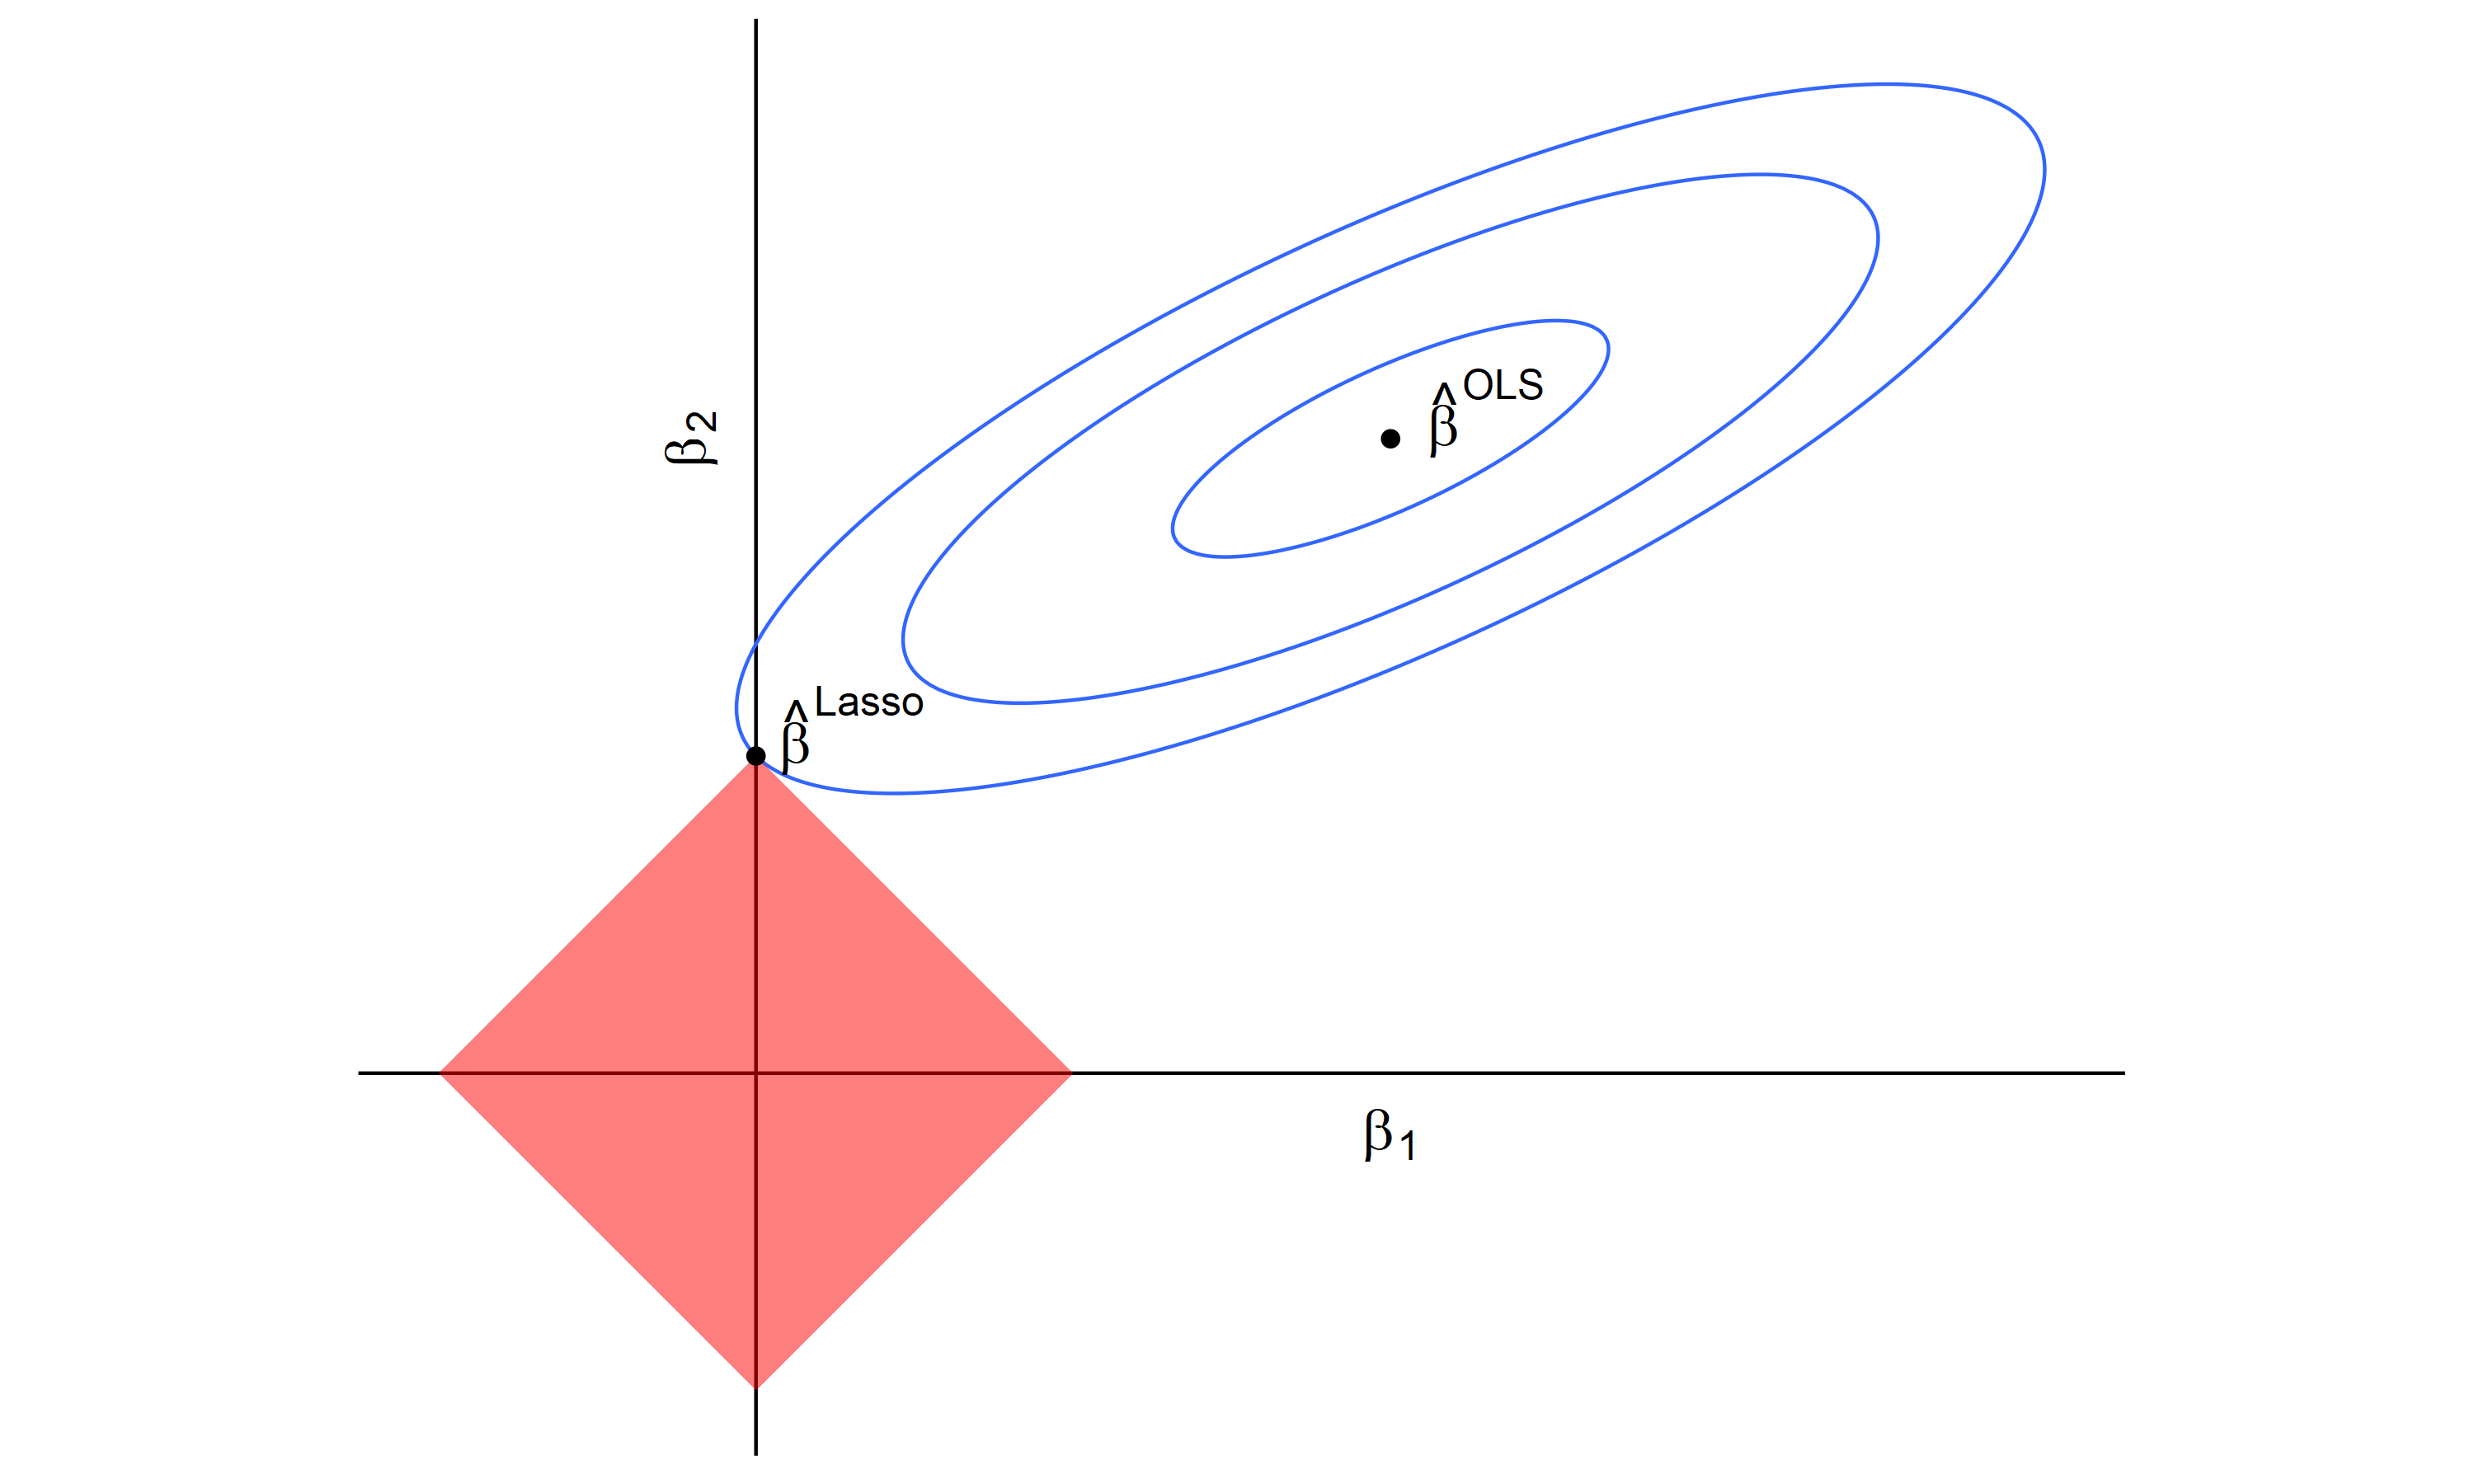
\includegraphics[width=\textwidth]{images/lasso-diagram.png}
	\end{subfigure}
	\captionsetup{width = 5in}
	\caption{RSS contours and penalty bounds for the ridge and LASSO models when $p=2$ and $t = 1$. The red regions represent the coefficient values allowed by ridge and LASSO regression, respectively. The blue ellipses represent contours of the residual sum of squares, with $\hat{\beta}^{\text{OLS}}$ being the point where the residual sum of squares is minimized. The intersection of the ellipse with the red region represents the point selected by LASSO and ridge.}
	\label{fig:ridge-lasso-diagram}
\end{figure}

\textbf{Elastic-net} regression uses both the ridge penalty and the LASSO penalty at the same time \cite{zou2005regularization}. Elastic-net solves the optimization problem
\begin{equation}
	\hat{\beta}^{\text{E-net}}=\argmin{\beta}{\sum\limits_{i = 1}^n \left( y_i - \beta_0 - \sum\limits_{i = 1}^p \beta_j x_{ij} \right) + \lambda_2\sum\limits_{j = 1}^p \beta_j^2 + \lambda_1\sum\limits_{j = 1}^p \vert \beta_j \vert}
\end{equation}
where $\lambda_1$ and $\lambda_2$ are both tuning parameters to be determined later.

An important limitation to note is that elastic net performs best when it close to either ridge or LASSO regression, meaning that either $\lambda_1$ greatly exceeds $\lambda_2$ or $\lambda_2$ greatly exceeds $\lambda_1$ \cite{zou2005regularization}. Additionally, because elastic net requires two tuning parameters, this makes it much more difficult to determine the best combination of tuning parameters to minimize error in the regression. However, this problem has been largely solved through by the LARS-EN algorithm developed by Zou et. al. which efficiently solves for the tuning parameters \cite{zou2005regularization}.

One major flaw of the LASSO method is that the penalty punishes large coefficients, even if those coefficients should be large. One way to modify the LASSO method is to use the \textbf{smoothly clipped absolute deviation} (SCAD) penalty \cite{fan2001variable}. The goal of this method is to punish large coefficients less severely, which can help mitigate some of the bias introduced by the LASSO method. The penalty function $P(\beta)$ for SCAD satisfies
\begin{equation}\label{eqn:scad-derivative-indicator}
	\frac{dP}{d\beta} = \cdot\sign(\beta)\left[ I(\vert \beta \vert<\lambda) + \frac{\max(a\lambda - \vert \beta\vert, 0)}{(a - 1)\lambda}I(\vert \beta \vert > \lambda) \right]
\end{equation}
where $a\geq 2$ is a new hyperparameter and $I$ is the indicator function ($I(Q)$ equals 1 if a statement $Q$ is true, and equals 0 if $Q$ is false). If the hyperparameter $a$ is large, then SCAD behaves like LASSO for larger coefficient values. Also, notice that $\lambda$ is an argument for the penalty function $P$.

An equivalent way to write the expression in Equation \ref{eqn:scad-derivative-indicator} is
\begin{equation}
	\frac{dP}{d\beta} = \left\{\begin{array}{ll}
		1,&\vert \beta \vert\leq \lambda\\
		\frac{a\lambda - \vert \beta \vert}{(a - 1)\lambda},&\lambda < \vert \beta \vert < a\lambda\\
		0,&\alpha\lambda < \vert \beta \vert
	\end{array}\right.
\end{equation}
This penalty function does not punish coefficients with large magnitude as heavily as the LASSO method. In fact, if the magnitude of a coefficient is larger than $a\lambda$, then the penalty becomes constant since the derivative becomes zero.

By integrating with respect to $\beta$ \cite{breheny2016lasso} and choosing $P(\beta) = 0$, we see that
\begin{equation}
	P(\beta) = \left\{\begin{array}{ll}
		\vert \beta \vert,&\vert \beta \vert \leq \lambda\\
		\frac{2a\lambda\vert\beta\vert - \beta^2-\lambda^2}{2(a - 1)\lambda},&\lambda < \vert \beta \vert < a\lambda\\
		\frac{\lambda(a + 1)}{2},&a\lambda < \vert \beta \vert
	\end{array}\right.
\end{equation}

The \textbf{minimax concave penalty} (MCP) method is very similar to SCAD \cite{zhang2010nearly, breheny2016lasso}. Both methods are used to avoid the high bias caused by the LASSO method. MCP uses a penalty function that satisfies
\begin{equation}
	\frac{dP}{d\beta} = \left\{\begin{array}{ll}
		\sign(\beta)\left(1 - \frac{\vert \beta \vert}{a\lambda}\right),& \vert \beta \vert \leq a\lambda\\
		0,&a\lambda < \vert \beta \vert
	\end{array}\right.
\end{equation}
where, like SCAD, $a>1$ is a hyperparameter. Integrating \cite{breheny2016lasso}, we see that
\begin{equation}
	P(\beta) = \left\{\begin{array}{ll}
		\vert \beta \vert - \frac{\beta^2}{2a\lambda},&\vert \beta \vert \leq a\lambda\\
		\frac{1}{2}a\lambda,&a\lambda < \vert \beta \vert
	\end{array}\right.
\end{equation}

Figure \ref{fig:lasso-scad-mcp} below shows the penalty functions (and their derivatives) for LASSO, SCAD, and MCP as a function of a coefficient value $\beta$. We see that LASSO applies a much stronger penalty to large coefficients than SCAD or MCP. Also, note that SCAD starts with a derivative equal to that of the LASSO for small values of $\beta$; on the other hand, the derivative of the penalty function for MCP starts decreasing immediately.

\begin{figure}[!h]
	\centering
	\begin{subfigure}[b]{0.4\textwidth}
		\caption{Penalty functions for LASSO, SCAD, and MCP}
		\label{fig:penalty}
		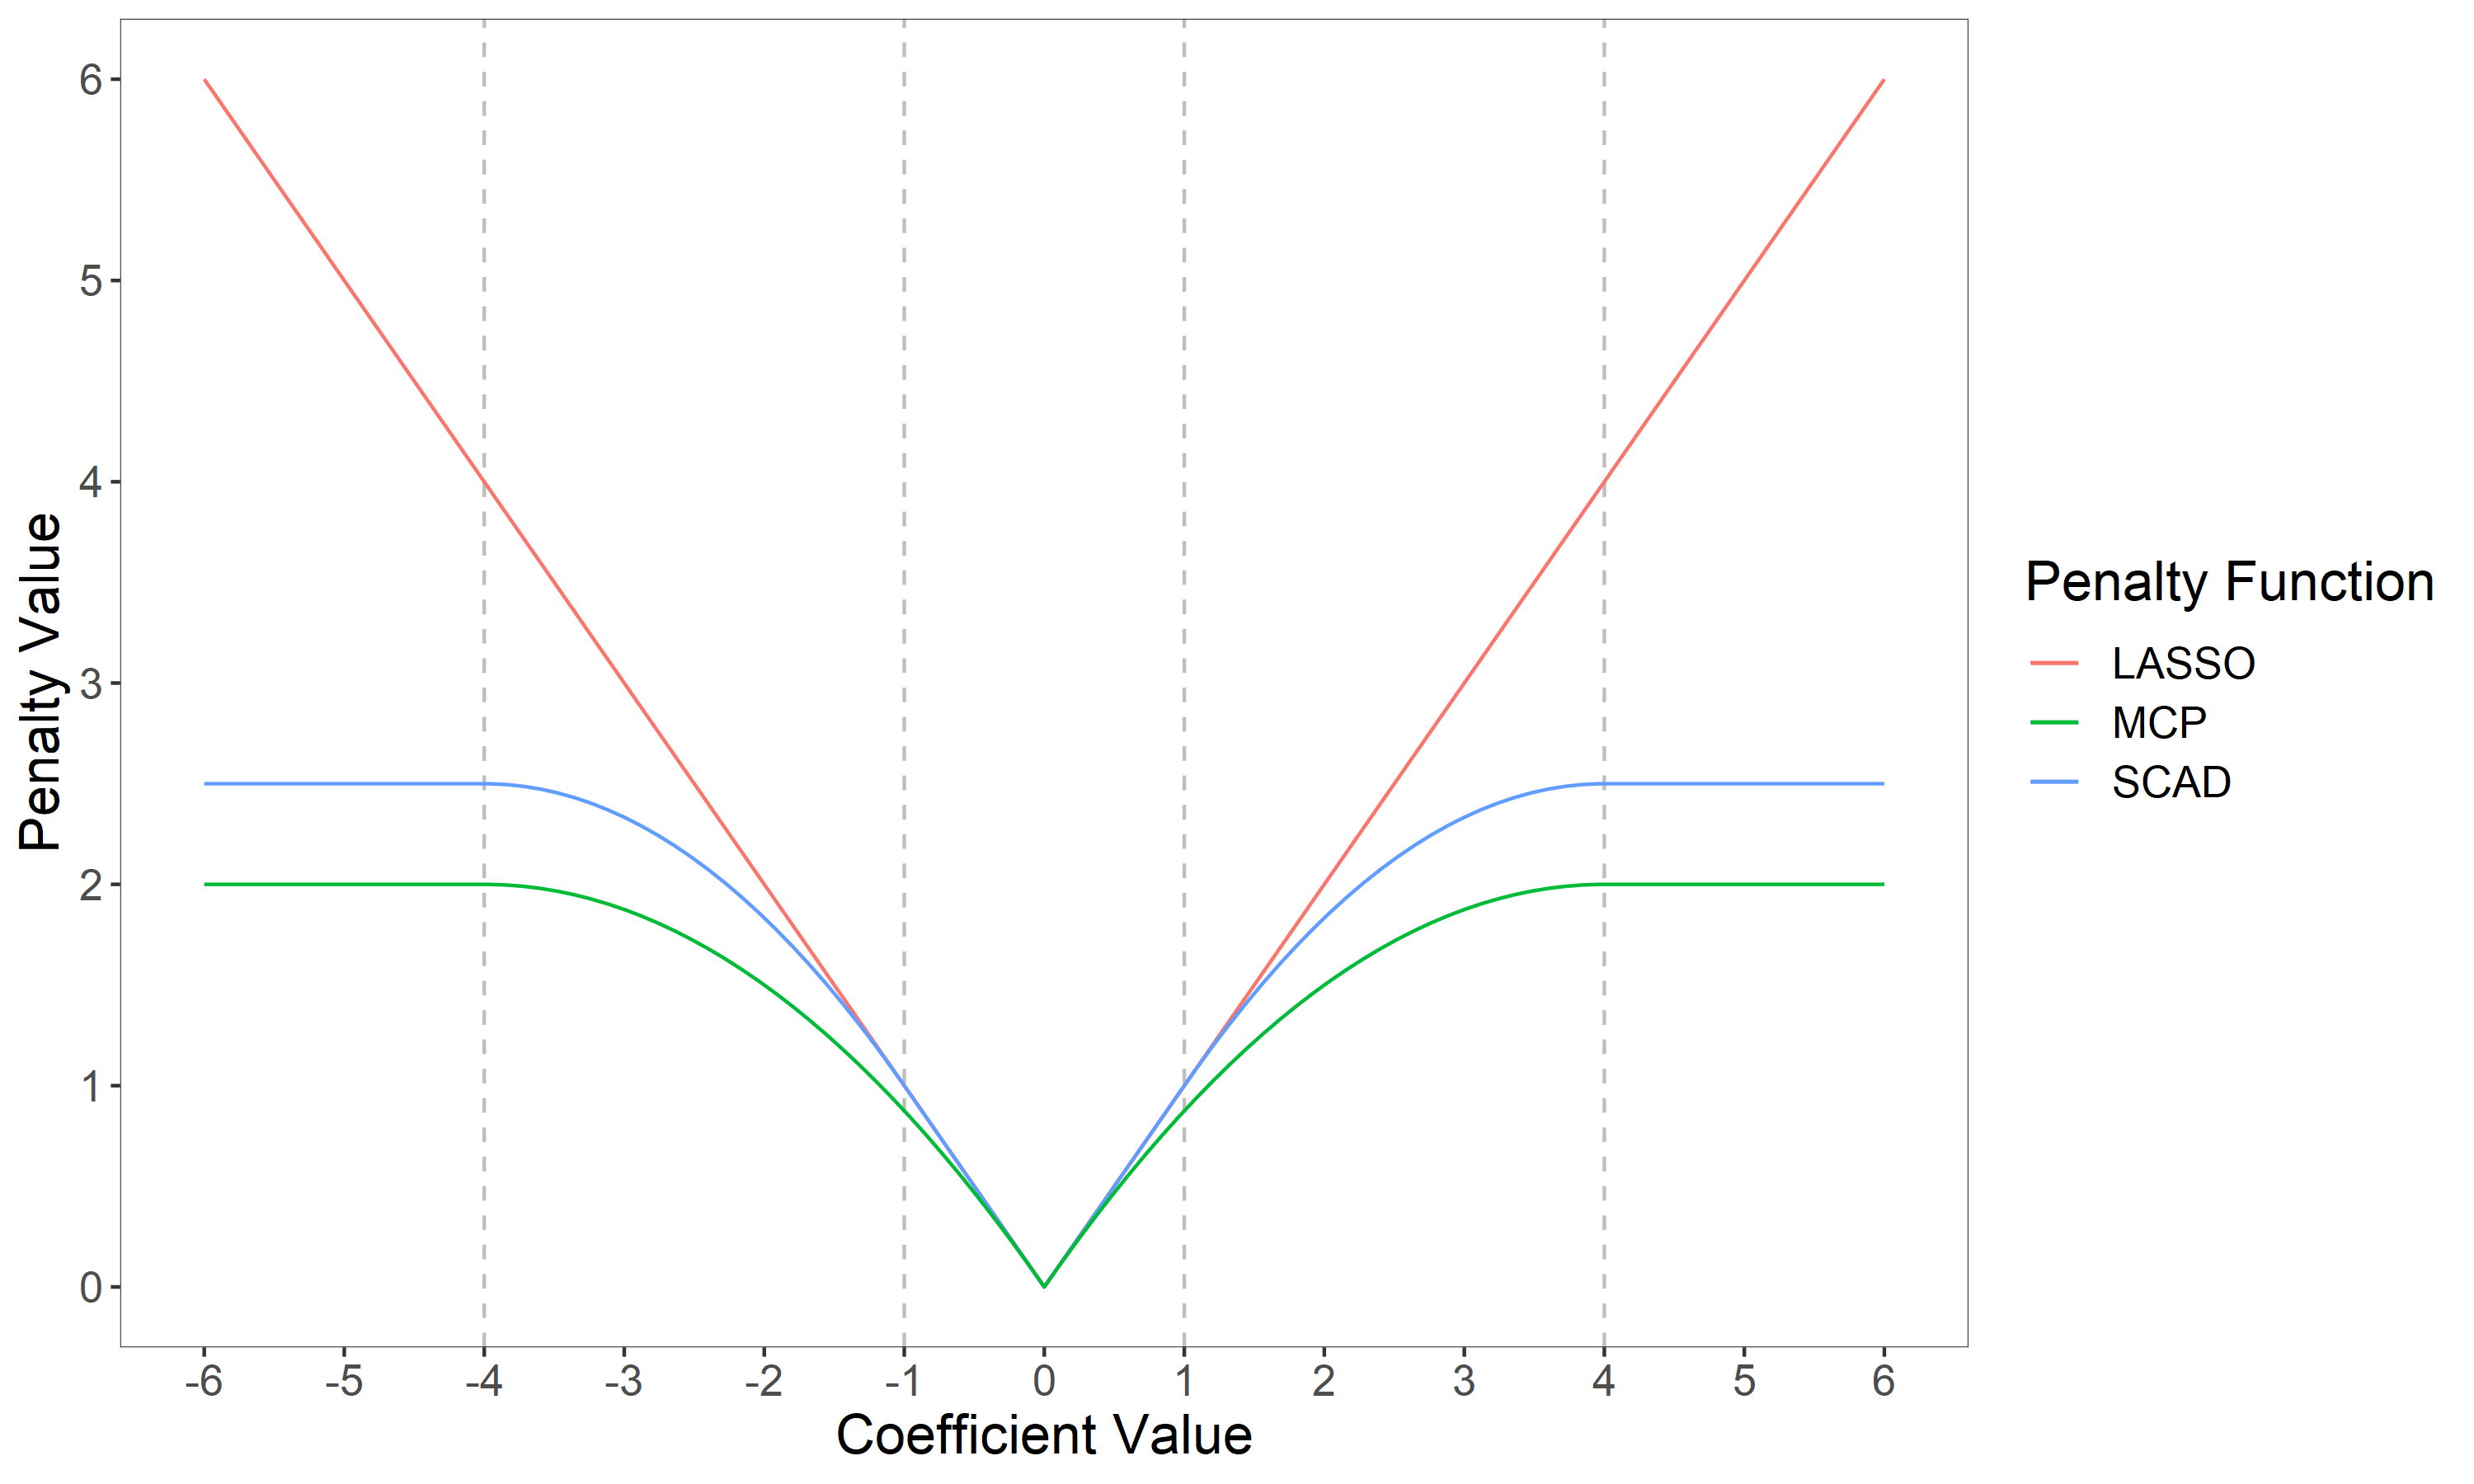
\includegraphics[width=\textwidth]{images/lasso-scad-mcp-penalty.png}
	\end{subfigure}
	\hspace{30pt}
	\begin{subfigure}[b]{0.4\textwidth}
		\caption{Derivatives of the penalty functions for LASSO, SCAD, and MCP}
		\label{fig:derivative}
		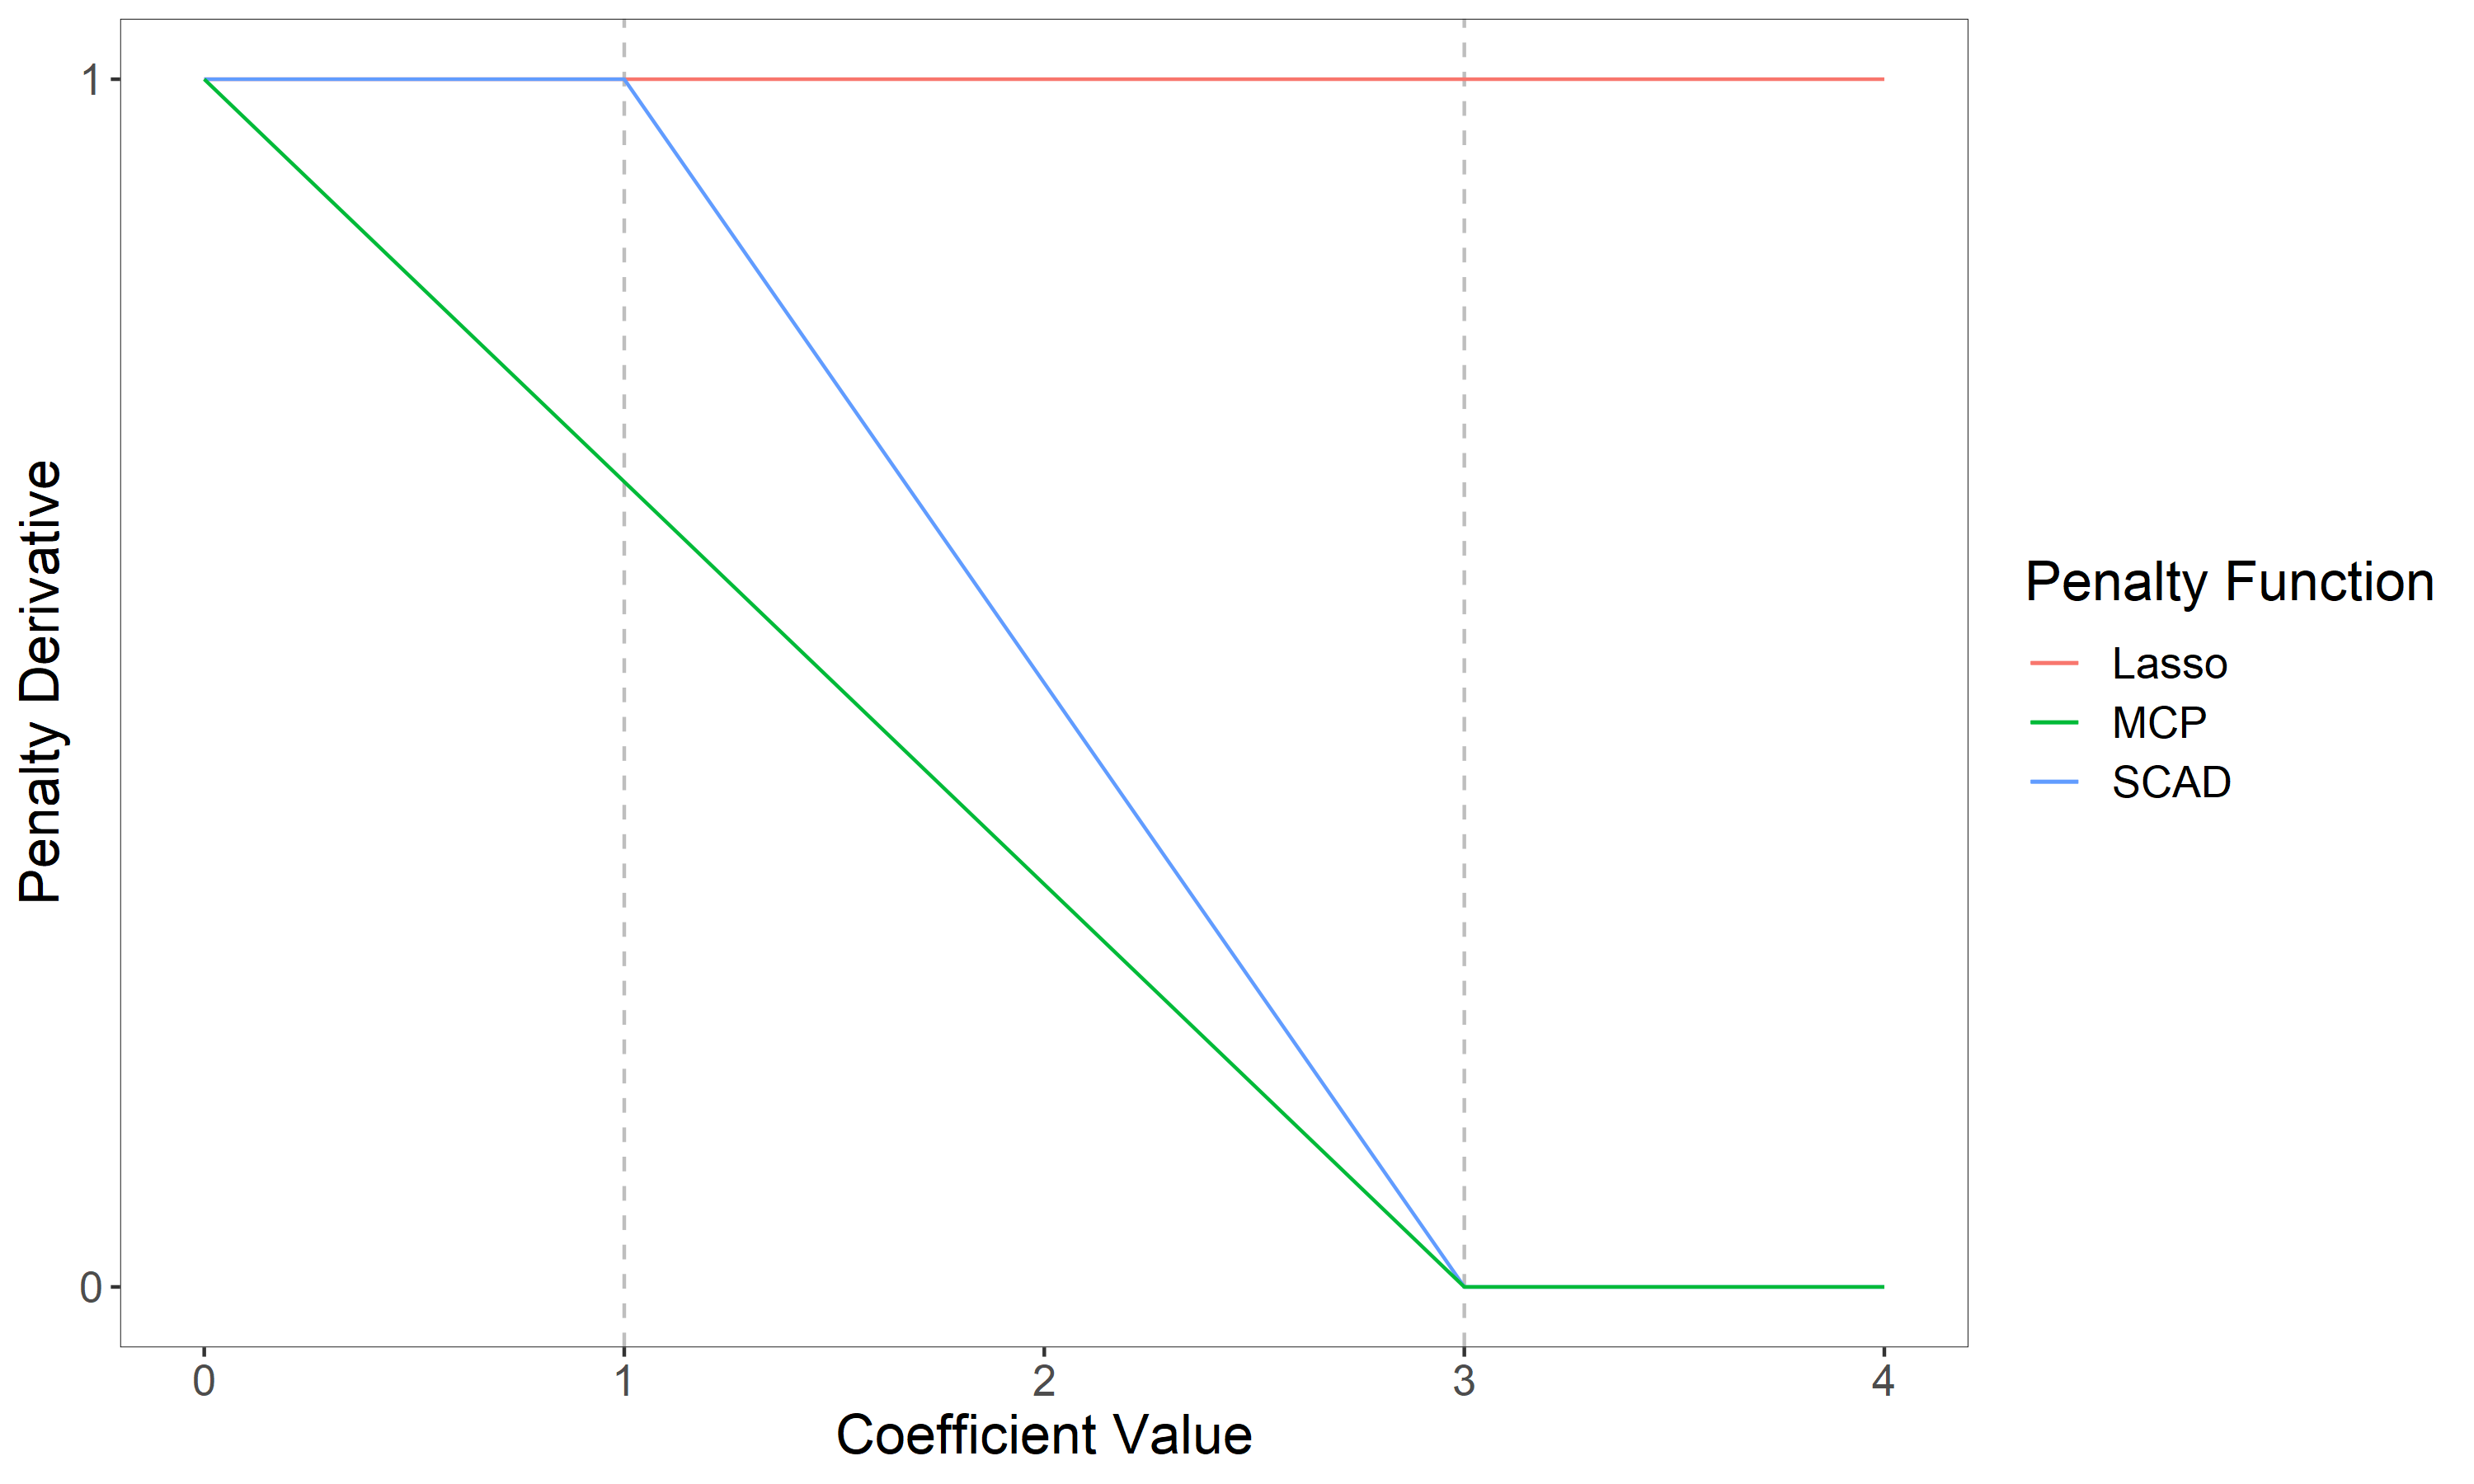
\includegraphics[width=\textwidth]{images/lasso-scad-mcp-derivative.png}
	\end{subfigure}
	\captionsetup{width = 5in}
	\caption{Penalty functions for LASSO, SCAD, and MCP, as well as their derivatives. These plots use $\lambda = 2$ and $a = 3$. The dashed vertical lines are the knots for SCAD and MCP.}
	\label{fig:lasso-scad-mcp}
\end{figure}

Note that of the penalized regression methods discussed above, only ridge regression has a general closed-form solution. Although LASSO, elastic-net, SCAD and MCP do not have closed-form solutions, their solutions can be efficiently approximated. In some special cases, however, a closed-form solution exists. 

Let $\mathbf{X}$ be a $n\times p$ matrix where each row contains the predictor values for one observation. To simplify things, we will assume that our data is centralized so that the coefficient $\beta_0$ is 0; that way, we do not need to include an extra entry of 1 in each row of $\mathbf{X}$. In an \textbf{orthonormal design}, we assume that $\mathbf{X}$ is orthonormal, meaning that the magnitude of each column of $\mathbf{X}$ is one and every pair of columns of $\mathbf{X}$ is orthogonal. In this special case, the value for each coefficient is independent of the other coefficients; in other words, we can compute each coefficient value as if it were the only predictor in the data set.

We can apply a \textbf{thresholding function} to each predictor to get the coefficient estimate for that predictor. For LASSO, elastic-net, SCAD, and MCP, a closed-form for this thresholding function exists \cite{tibshirani1996regression, fan2001variable, zou2005regularization, zhang2010nearly}. The input to the thresholding function is the actual coefficient value, and the output is the estimated value for that coefficient in an orthonormal design. Figure \ref{fig:prediction} shows the threshold functions for LASSO, SCAD and MCP when $\lambda = 2$ . For SCAD and MCP, we used the value $a = 3$. For reference, the identity line is included, which can be considered as the threshold function for ordinary least squares.

Another feature of SCAD and MCP is that they

\begin{figure}[!h]
	\centering
	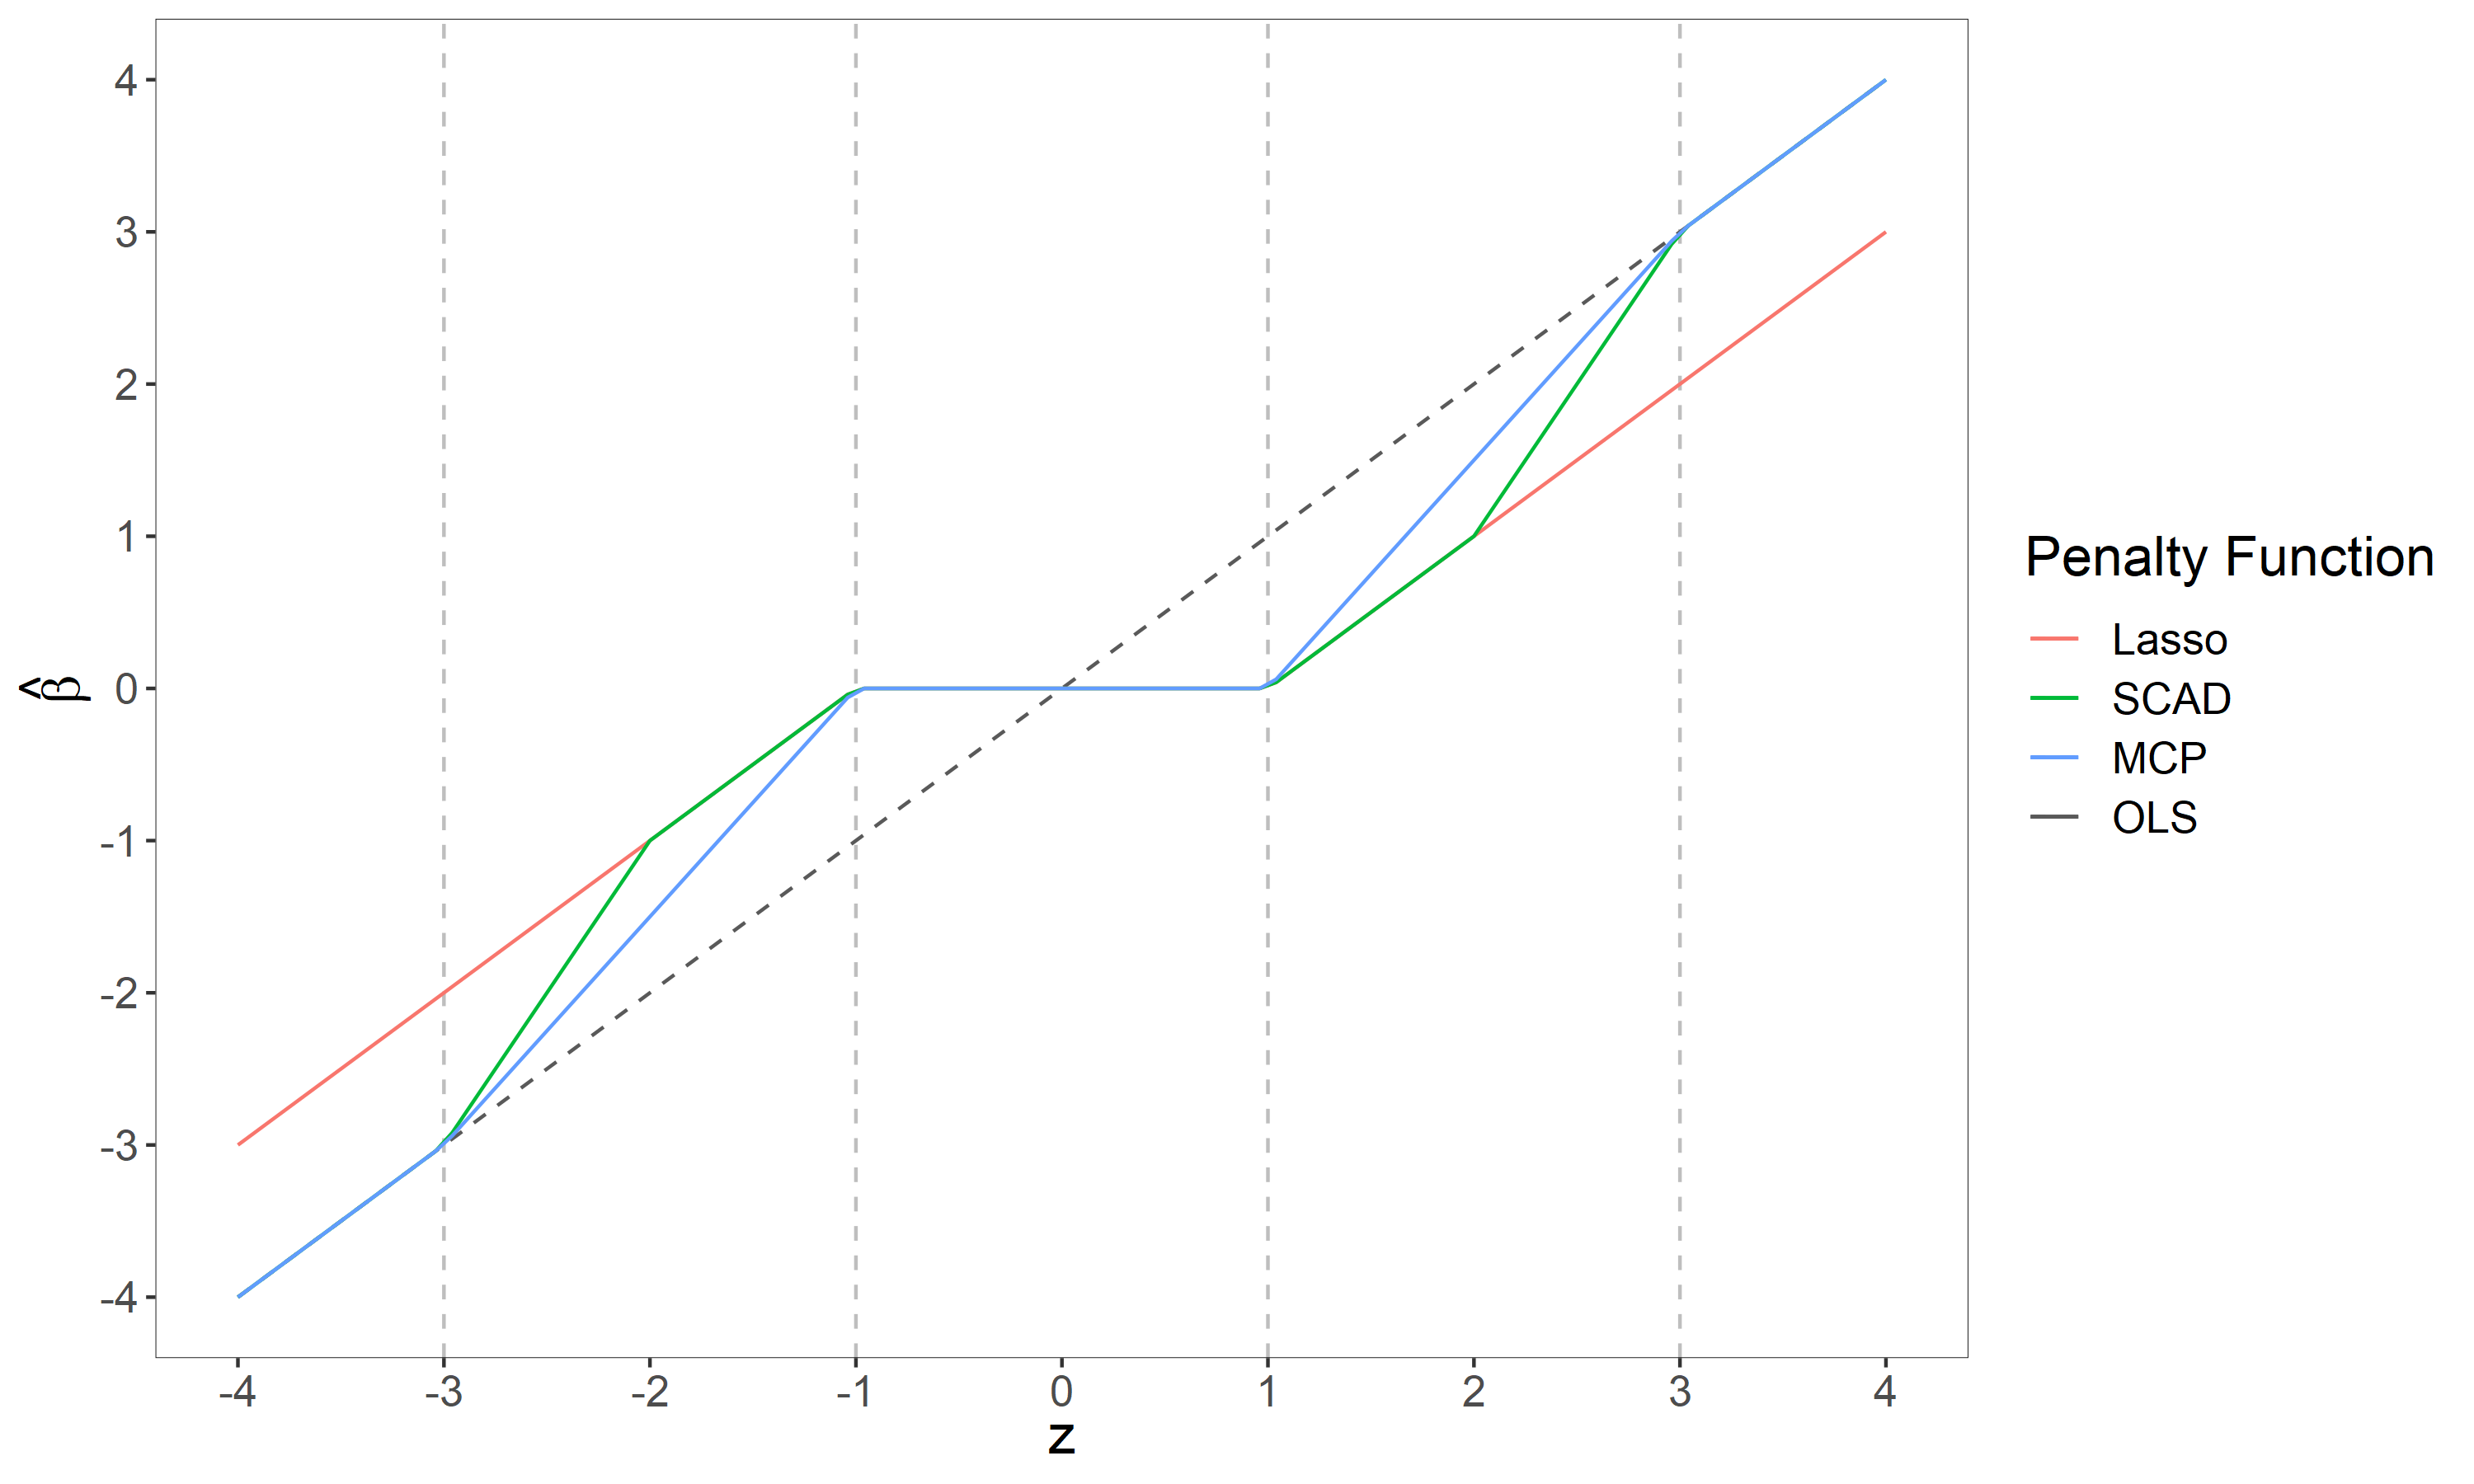
\includegraphics[width = 0.4\textwidth]{images/lasso-scad-mcp-solution.png}
	\captionsetup{width = 4in}
	\caption{Thresholding function for LASSO, SCAD, and MCP when $\lambda = 2$ and $a = 3$. In an orthonormal design, this function can be applied to the true coefficient values to get the predicted coefficient values. The dashed vertical lines are the knots for SCAD and MCP.}
	\label{fig:prediction}
\end{figure}

We see that when $\vert \beta \vert$ is small, the thresholding function for LASSO, SCAD, and MCP are all zero. This matches with the assumption that these methods should set small coefficient values to zero. As $\vert \beta \vert$ increases, the estimated value for that coefficient gets larger. Notice that ordinary least squares doesn't decrease the estimated coefficient value for any choice of $\beta$; this is because of the fact that ordinary least squares is unbiased, whereas the other methods are biased.

In this figure, we also see that the threshold function for LASSO is parallel to the identity line for large values of $\beta$. This means that even if a predictor is very influential on the response, LASSO will predict a coefficient estimate that is less than the true coefficient value. This makes LASSO a very biased model. This issue was one of the main motivations for SCAD and MCP. Unlike LASSO, SCAD and MCP converge to the identity line as $\beta$ increases, which makes these methods less likely to decrease large coefficient estimates.

Another feature of SCAD and MCP is their \textbf{oracle-like properties}. In this context, the term \textbf{oracle} comes from a paper by Donohe and Johnstone about spatially variable estimators \cite{donoho1994ideal}. They consider an ideal situation where a model could be fitted with the aid of an oracle. This oracle could give information about the underlying behavior of the function $f$ relating a response variable to the predictors without giving the function $f$ itself.

In the context of linear regression, an oracle estimator would know which predictors are truly correlated with the response. With the aid of an oracle, one could then fit an ordinary least squares model using only the coefficients that are actually non-zero and ignoring the predictors that are actually zero. Fan and Li in \cite{fan2001variable} and Zhang in \cite{zhang2010nearly} prove that SCAD and MCP both have oracle-like properties. Under certain conditions, SCAD and MCP can perform as well as the oracle estimator as $n$ approaches $\infty$. On the other hand, LASSO does not have oracle-like properties, meaning that its predictions cannot perform as well as a model found with the aid of an oracle.

\subsection{Non-linear models}
We next discuss several non-linear methods for regression: random forests, gradient boosting, and support vector machines.

Both random forest and gradient boosting models use \textbf{decision trees} to make predictions. A decision tree is a binary tree where each non-leaf node represents a condition and each leaf node represents a prediction value. To make a prediction, start at the root node and check whether the condition at that node is true or false. If true, move down to the node's first child; if false, move to the second child. This process is repeated until a leaf node is reached. This node will give a value that the decision tree predicts.

Although decision trees can be used as machine learning models on their own, it is more common to use decision trees in ensemble methods, which combine many different decision trees into a single model. A single decision tree will usually have high variance since a small change in the training set can lead to a completely different decision tree \cite{james2013introduction}.

\textbf{Random Forests} solve the issue of high variance by aggregating the predictions of many independent decision trees. Each tree is fit using a subset of the observations and a subset of the predictors, so that the trees are relatively independent from one another.

To generate a tree within a random forest model, first select a random sample of the $n$ observations with replacement. This is a process called \textbf{bootstrapping}. The number of observations chosen for each tree is a hyperparameter that can be changed. After selecting a set of observations, a random sample of predictors are chosen out of the $p$ predictors without replacement. Again, this helps decorrelate the trees. The number of predictors used in each tree is also a hyperparameter that can be changed. Then, a decision tree is generated using the available observations and predictors. The number of trees generated is another hyperparameter; usually, a random forest model will contain at least several hundred trees.

To make predictions with a random forest, a test observation is passed into each decision tree and the predictions from each tree are aggregated. For regression, the results are normally aggregated using the mean; for classification, the prediction chosen most often by the trees is usually used as the final prediction.

\textbf{Boosting} is the technique of sequentially improving a weak learner until it becomes a strong learner. A \textbf{gradient boosting model} (GBM) is a boosting technique that uses gradient descent to minimize error in a model and correct the shortcomings of the previous weak learner model. This is done through fitting a model, whether that is a linear regression or decision tree model, to a set of data points. From there, the residual of each data point is calculated and another linear regression or decision tree model is fitted to those residuals. A new model is fitted to the residual data of the residual data fitted model, and so on. These models are then all added together to result in a strong GBM model.

Gradient boosting can be used for both regression and classification if they use decision trees, or if they use linear regression models, they can only perform regression. When using a gradient boosting model with decision trees, variable importance and pruning can be used as a sort of pseudo-variable selection method to lower complexity and prevent over-fitting. However, when using a gradient boosting model with linear regression, there is the ability to use lasso, ridge, and elastic net penalized regression as the weak learner and perform variable selection.

Gradient boosting models often suffer from slow computation speeds due to the large number of sequential models that need to be trained. \textbf{Extreme Gradient Boosting} (XGBoost) is a faster version of gradient boosting that utilizes parallel computing as well as different optimization techniques to speed up computation. For these reasons, XGBoost is often preferred over standard gradient boosting models and is very commonly used in many machine learning applications.

For our study, we considered a few different hyperparameters. The learning rate controls how quickly the gradient boosting model learns. If this learning rate is high, then the model learns quickly, but it may not learn as efficiently. If the learning rate is low, then the model takes longer but typically makes better predictions. The maximum tree depth determines how high each tree can be. Using smaller tree sizes may oversimplify the model, but it could also mitigate overfitting.

\textbf{Support vector machines} are versatile statistical models that can be used for both regression and classification. In the ideal case, a support vector machine is a binary classier whose decision boundary is a $(p-1)$-dimensional hyperplane in $p$-dimensional space that perfectly separates all of the observations for one class on one side and the observations for the other class lie on the opposite side. Moreover, the hyperplane chosen by a support vector machine will maximize the distance between this hyperplane and any of the observation points.

However, most data sets cannot be split perfectly into two sides. Furthermore, this model has very high variance as changing the points near the hyperplane can significantly alter the hyperplane. Finally, this model cannot handle cases where the true boundary is non-linear. Luckily, support vector machines in practice can handle such issues. Typically, support vector machines are allowed to misclassify some of the training data, which address the cases where the data cannot be split perfectly by a hyperplane. Also, the predictor space can be enlarged to handle non-linear decision boundaries; this is typically done by using \textbf{kernels}. For example, using a radial kernel can create decision boundaries that enclose regions of the $p$-dimensional space.

Although support vector machines are usually used for classification, they can be generalized to perform regression as well. We will be using support vector machines for regression in our study.

Like the other non-linear methods, there are many hyperparameters that can be tuned. The two hyperparameters that we considered are $\epsilon$ and the cost function. $\epsilon$ defines how tolerant the algorithm is of small errors. If $\epsilon$ is large, then the support vector machine will tolerate larger errors; if $\epsilon$ is small, then even small errors will be punished. The cost hyperparameter $C$ determines how strongly the model punishes incorrect predictions. If $C$ is large, then the model punishes incorrect predictions more, making it fit more tightly to the training set. If $C$ is smaller, then the model is likely to allow more incorrect predictions in the training data.

%%%%%%%%%%%%%%%%%%%%%%%%%%%%%%%%%%%%%%%%%%%%%%%%%%%%%%%%%%%%%%%%%%%%%
\section{Methods}
To test and evaluate each of the models discussed above, we considered both Monte Carlo simulations and empirical data. Monte Carlo simulations allow us to test the models under different environments to get a comprehensive idea of how each model performs. Furthermore, by repeating each simulation many times, our results will be more consistent than if we just relied on one data set to test each model.

For our empirical data analysis, we used
\subsection{Models}
% lists and describes every tested model. Can include equations for models, but should not go into such great depth about each model: that can be reserved for literature review portion of the paper.

\subsection{Monte Carlo Simulations}
% outline data generation process and factorial design process

Monte Carlo simulations use randomly generated data to fit and test our regression and classification models. There are several benefits to using simulated data rather than experimental data:
\begin{itemize}
	\item The true relationship between the predictor variables and the response is known.
	\item Simulations can be iterated many times, giving sturdier results about the effectiveness of each model.
	\item We have full control over factors such as the number of predictors and the amount of correlation between predictors.
\end{itemize}

For the simulated data, we assumed that the relationship between the response variable $y$ and the predictors $x_1, x_2, \dotsc, x_p$ was linear. That is, we assumed that
\begin{equation}
	y = \beta_0 + \beta_1 x_1 + \cdots + \beta_p x_p + \epsilon
\end{equation}
where $\beta_0$ is some intercept, $\beta_1, \dotsc, \beta_p$ are coefficient values and $\epsilon\sim \mathcal{N}(0, \sigma^2)$ is a normally distributed random error with mean 0 and variance $\sigma^2$.

To generate the data, we first defined $\beta = [\beta_0, \beta_1, \dotsc, \beta_p]^\top$, a $(p + 1)\times 1$ vector of coefficient values. For our simulations, we used $\beta_0 = 1$, $\beta_1 = 2$, $\beta_2 = -2$, $\beta_5=0.5$ and $\beta_6 = 3$; the remaining coefficient values were set to 0.

Next, we generated $\mathbf{X}$, a $n\times (p + 1)$ matrix of predictor variables. The first column contains 1 in all of its entries; this corresponds to the intercept of our linear model. Column $i$ of $\mathbf{X}$ contains the variable values for predictor $x_{i - 1}$, for $1\leq i\leq p$. These values were generated using the $p$-dimensional multivariate normal distribution $\mathcal{N}_p(0, \mathbf{\Sigma})$ with mean zero and covariance matrix $\mathbf{\Sigma}$. We assumed that every predictor had a standard deviation of 1, making the covariance matrix equivalent to a correlation matrix. Four different correlation matrix structures were considered in our study.

We then generated an $n\times 1$ error vector $\mathbf{e}\sim \mathcal{N}(0, \sigma^2)$ with mean zero and variance $\sigma^2$. For regression models, the response $\mathbf{y}$ can then be computed by
\begin{equation}
	\mathbf{y} = \mathbf{X}\beta + \mathbf{e}
\end{equation}

We used a \textbf{factorial design} for our simulations. This means that we considered several factors that affect the data generation process, each having multiple possible values. We then generated data using every possible combination of factor values, giving us a comprehensive assessment of model performance under various conditions.
\begin{itemize}
	\item $n$, the number of observations: 50, 200, 1000.
	\item $p$, the number of predictors: 10, 100, 2000.
	\item $\sigma$, the standard deviation of the random error: 1, 3, 6.
	\item The correlation matrix structure: independent, symmetric compound, autoregressive, blockwise.
	\item $\rho$, the correlation between predictors: 0.2, 0.5, 0.9.
\end{itemize}

By taking every possible combination of these factors, we obtain $3\times 3\times 3\times 4\times 3 = 324$ different settings for the simulations. However, because an independent correlation matrix does not use the correlation value $\rho$, we actually only used 270 combinations. For each combination of factors, we ran 100 simulations. In each simulation, we generated two data sets: one to train the various models, and one to test the models and evaluate performance. Both data sets contained $n$ observations, meaning that a total of $2n$ observations were generated for each simulation.

As mentioned earlier, we considered four different covariance matrix structures. These structures determine the correlation between different predictors. If $\mathbf{\Sigma}$ is a correlation matrix, then $\mathbf{\Sigma}_{ij}$, the entry at the $i$-th row and $j$-th column, represents the correlation between predictors $i$ and $j$. If $\mathbf{\Sigma}_{ij}=0$, there is no correlation; but if $\mathbf{\Sigma}_{ij}=1$, then predictors $i$ and $j$ are perfectly correlated. Note that a correlation matrix is always symmetric, so $\mathbf{\Sigma}_{ij} = \mathbf{\Sigma}_{ji}$ for all indices $i$ and $j$. This correlation can severely impact the performance of statistical models; if several predictors are highly correlated, then machine learning algorithms are less able to determine which predictors are actually related to the response.

The first correlation structure we considered is \textbf{independent correlation}. This means that the correlation matrix $\mathbf{\Sigma}$ has the form
\begin{equation}
	\mathbf{\Sigma} = \begin{bmatrix}
		1 & 0 & \cdots & 0 \\
		0 & 1 & \cdots & 0 \\
		\vdots & \vdots & \ddots & \vdots \\
		0 & 0 & \cdots & 1
	\end{bmatrix}
\end{equation}
In other words, there is no correlation between different predictors, since $\mathbf{\Sigma}_{ij} = 0$ whenever $i\neq j$. Although this is a very simple case, it is very unrealistic.

The next covariance structure is called \textbf{symmetric compound}. This structure has the form
\begin{equation}\label{eqn:symmetric-compound-matrix}
	\mathbf{\Sigma} = \begin{bmatrix}
		1 & \rho & \cdots & \rho \\
		\rho & 1 & \cdots & \rho \\
		\vdots & \vdots & \ddots & \vdots \\
		\rho & \rho & \cdots & 1
	\end{bmatrix}
\end{equation}
where $\rho \in [0, 1]$ is some correlation value. A symmetric compound covariance structure assumes that $\mathbf{\Sigma}_{ij} = \rho$ whenever $i \neq j$, meaning that all predictors are equally correlated with one another. By introducing correlation between different predictors, the data generated in our simulations is more realistic. However, a symmetric compound covariance matrix is still relatively simplistic. In real data sets, it is unrealistic to assume that all of the predictors have the exact same correlation with one another.

An autoregressive covariance structure assumes that
\begin{equation}
	\mathbf{\Sigma} = \begin{bmatrix}
		1 & \rho & \cdots & \rho^{p - 1} \\
		\rho & 1 & \cdots & \rho^{p - 2} \\
		\vdots & \vdots & \ddots & \vdots \\
		\rho^{p - 1} & \rho^{p - 2} & \cdots & 1
	\end{bmatrix}
\end{equation}
For any indices $i$ and $j$, we have $\mathbf{\Sigma}_{ij} = \rho^{\vert i - j\vert}$. Consequently, each predictor is strongly correlated with nearby predictors and weakly correlated with more distant predictors. This form of covariance is commonly seen when using time series, since observed values at nearby times are likely to be highly correlated with one another. 

Finally, a blockwise correlation matrix has the block-diagonal form
\begin{equation}
	\mathbf{\Sigma} = \begin{bmatrix}
		\mathbf{B}_1 & 0 & \cdots & 0 \\
		0 & \mathbf{B}_2 & \cdots & 0 \\
		\vdots & \vdots & \ddots & \vdots \\
		0 & 0 & \cdots & \mathbf{B}_k
	\end{bmatrix}
\end{equation}
where $0$ represents a block containing all zeroes, and each block $\mathbf{B}_i$ has a form identical to the symmetric compound matrix in Equation \ref{eqn:symmetric-compound-matrix}. This implies that predictors within the same block have correlation $\rho\in [0, 1]$, whereas predictors in different blocks have zero correlation. This type of correlation is more realistic than independent or symmetric compound correlation, since only certain groups of predictors are correlated with one another. One important consideration when using blockwise correlation is the size of each block. For our simulations, we used a block size of 5 when $p = 10$, a block size of 25 when $p = 100$, and a block size of 100 when $p = 2000$.

All of our simulations were run using version 4.1.0 of \lstinline!R!. Several different libraries were used to fit machine learning models using our simulated data. Table \ref{tab:model-libraries} summarizes the libraries used to fit models.

\begin{table}[h]
	\centering
	\caption{\lstinline!R! Libraries used and the models used from each library}
	\label{tab:model-libraries}
	\begin{tabular}{lll}\hline
		\textbf{Library}    & \textbf{Models used}                                 & \textbf{Version} \\ \hline
		\lstinline!stats!   & Ordinary least squares                               & 4.1.0            \\
		\lstinline!MASS!    & Forward and backward selection                       & 7.3-54           \\
		\lstinline!glmnet!  & Ridge, lasso, elastic-net                            & 4.1-1            \\
		\lstinline!gcdnet!  & Adaptive ridge, adaptive lasso, adaptive elastic-net & 1.0.5            \\
		\lstinline!ncvreg!  & SCAD and MCP                                         & 3.13.0           \\
		\lstinline!xgboost! & Gradient boosting                                    & 1.4.1.1          \\
		\lstinline!ranger!  & Random forest                                        & 0.12.1           \\
		\lstinline!e1071!   & Support vector machine                               & 1.7-7            \\\hline
	\end{tabular}
\end{table}

For ridge, lasso, and elastic-net regression using \lstinline!glmnet!, we used the \lstinline!cv.glmnet! function. This function uses cross-validation to determine the value of $\lambda$ that minimizes the cross-validation error. We used ten folds with \lstinline!cv.glmnet!. Using cross-validation can help generate a model that has a good test performance. For elastic-net regression, we used the hyperparameter $\alpha = 0.8$. This means that the elastic-net model is more similar to lasso (where $\alpha = 1$) than ridge (where $\alpha = 0$). The remaining hyperparameters were given their default values.

We used the \lstinline!cv.gcdnet! function from the \lstinline!gcdnet! library for the adaptive versions of ridge, lasso, and elastic-net. Again, ten folds were used for the cross-validation, and all hyperparameters were given their default values.

For SCAD and MCP models, we used the \lstinline!cv.ncvreg! function from the \lstinline!ncvreg! library. We used the default values of $a$ for both models: 3 for MCP and 3.7 for SCAD (note that the \lstinline!ncvreg! documentation calls this hyperparameter $\gamma$ instead of $a$).

For the three non-linear models (gradient boosting, random forests, and support vector machines), we used cross-validation and grid search to find suitable hyperparameters, and then fit a model using the full training set using those hyperparameters. For gradient boosting with \lstinline!xgboost!, we used different values for the learning rate (0.1, 0.3, and 0.5) and maximum tree depth (1, 3, and 7). A maximum of 1000 trees were generated, with an early stopping condition if the model failed to improve for several iterations in a row. The cross-validation function used five folds.

For random forests using \lstinline!ranger!, we tuned the number of predictors used per decision tree ($\lfloor \sqrt{p}\rfloor$, $\lfloor p / 3 \rfloor$, and $\lfloor p / 2 \rfloor$) and the number of trees (300, 400, 500 and 600). The cross-validation function used five folds.

Finally, for support vector machines using \lstinline!e1071!, we varied $\epsilon$ (TODO: explain this) and the cost function (0.5, 1, and 2).




\subsection{Empirical Data}
% outline empirical data sources and what each database is about / what we try to predict about it

For empirical data, we used the Breast Cancer database from The Cancer Genome Atlas (bcTCGA). This contains the gene expression data of 17323 genes from 536 patients. One of these genes is the BRCA1 gene which is among the first genes discovered that can increase the risk of breast cancer. Because the BRCA1 gene interacts with other genes, it is useful to find genes that interact with BRCA1 to test in further studies. The distribution of the BRCA1 gene expression levels in the bcTCGA database can be seen in Figure \ref{fig:BRCA1-distribution}. The BRCA1 gene expression level will act as the output value in our regression analysis and the other 17322 genes will serve as predictor values.

\begin{figure}[h!]
	\centering
	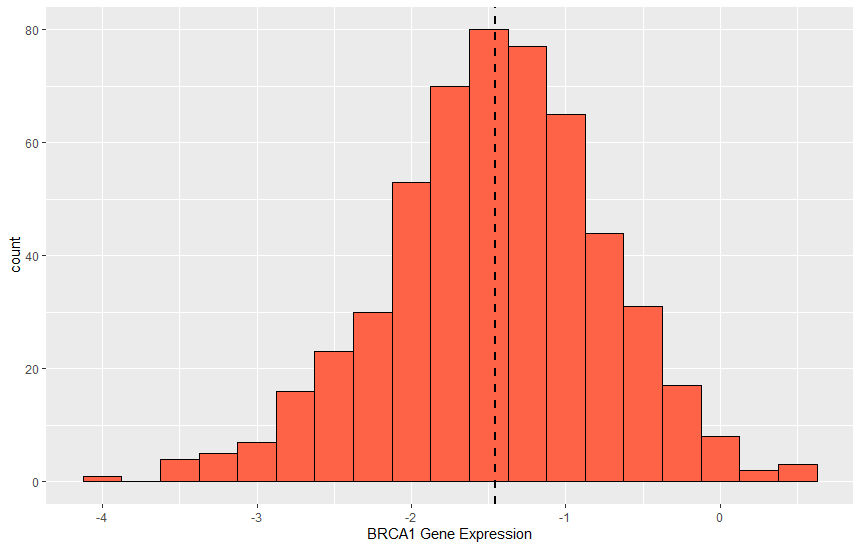
\includegraphics[width = 0.7\linewidth]{images/BRCA1-expression.png}
	\caption{Distribution of BRCA1 gene expression levels}
	\label{fig:BRCA1-distribution}
\end{figure}

This data is a prime example of the $p>>n$ problem where there are many more predictors than data samples. Because of this, only penalized regression and machine learning techniques can be utilized. This is because there are more predictors than samples which makes least squares linear regression impossible and due to the high number of predictors, subset and stepwise regression becomes too computationally expensive to be feasible. Additionally, support vector machines struggle at such a high number of predictors and resulted in stack overflow errors which made fitting support vector machines on this data infeasible.

For analyzing the error of models fitted using this empirical data, we performed nested cross validation. Many of the models fitted used cross validation for tuning purposes to find the best input parameters. Examples of these parameters include $\lambda$ for penalized regression techniques, the number of trees and number of predictors for random forest, as well as max depth and learning rate for XGBoost. However, we also perform 5-fold cross validation before we even allow the models to tune their parameters. By doing nested cross validation, testing data is not used for training the model \textbf{or} tuning model parameters. This results in a more accurate error calculation. If nested cross validation was not used, models could tune their parameters in a way that overfits the model to the testing data which would lead to artificially decreased error and invalid results.
%%%%%%%%%%%%%%%%%%%%%%%%%%%%%%%%%%%%%%%%%%%%%%%%%%%%%%%%%%%%%%%%%%%%%
\section{Results}


\subsection{Monte Carlo Simulations}
% stick the results from logisitc regression and classification models here

Because we ran simulations using 270 different combinations of factors, we will just highlight some results.

\subsection{Empirical Data}
% Stick all the results from the linear regression models here

\begin{figure}[h!]
	\centering
	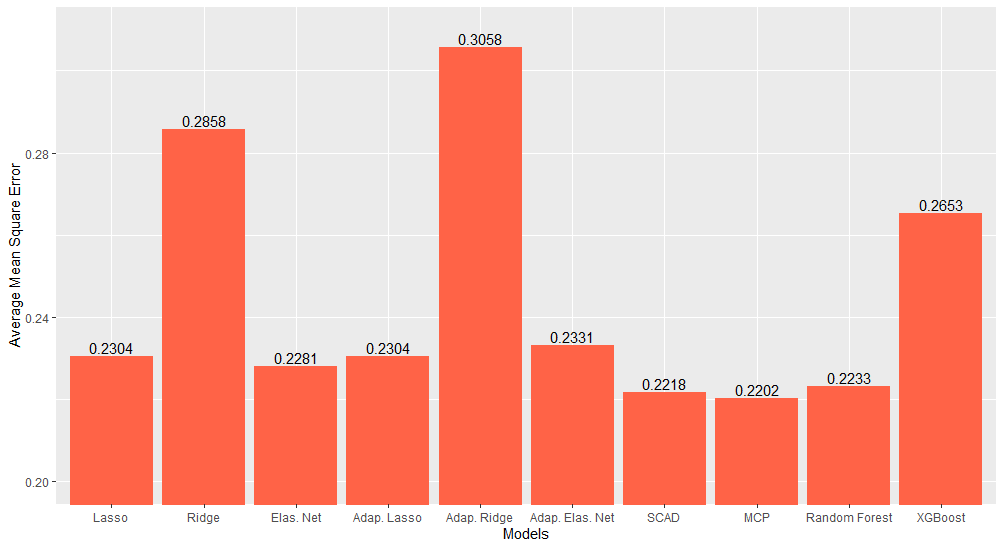
\includegraphics[width = 0.9\linewidth]{images/empirical_cv_mse.png}
	\label{fig:empirical_mse}
	\caption{Average Mean Square Error for Empirical Data Models}
\end{figure}
%%%%%%%%%%%%%%%%%%%%%%%%%%%%%%%%%%%%%%%%%%%%%%%%%%%%%%%%%%%%%%%%%%%%%
\section{Discussion}
% discussion of findings, future work, and contributions
\subsection{Findings}
% overall ideas that we found out after all these results. Which type of model is best in which environment, etc?
% Might need to break it into sub sub sections for classification vs regression or monte carlo vs empirical???
\subsection{Contributions}
% what are our contributions, why is what we did important?
% we have a comprehensive analysis of 21 models in 270 different environments. Allows for comprehensive comparison and gives guidance to data scientists as to which model they should use for their research
% empirical data methods show the important uses of penalized regression in environmental, biological, and etc. data
\subsection{Future Work}
% maybe talk about the penalty method we came up with? Talk about how it might be able to solve issues of Logsum method?

\newpage
\appendix

\setlength{\tabcolsep}{4pt}
{\tiny
\begin{adjustbox}{angle=90}
\begin{tabular}{llllllllllllllllllllll}
	\hline
	& & \multicolumn{20}{l}{type} \\ 
	& & \multicolumn{2}{l}{independent} & \multicolumn{6}{l}{symmetric} & \multicolumn{6}{l}{autoregressive} & \multicolumn{6}{l}{blockwise} \\ 
	& & \multicolumn{2}{l}{corr} & \multicolumn{6}{l}{corr} & \multicolumn{6}{l}{corr} & \multicolumn{6}{l}{corr} \\ 
	& & \multicolumn{2}{l}{0} & \multicolumn{2}{l}{0.2} & \multicolumn{2}{l}{0.5} & \multicolumn{2}{l}{0.9} & \multicolumn{2}{l}{0.2} & \multicolumn{2}{l}{0.5} & \multicolumn{2}{l}{0.9} & \multicolumn{2}{l}{0.2} & \multicolumn{2}{l}{0.5} & \multicolumn{2}{l}{0.9} \\ 
	& & \multicolumn{2}{l}{test.mse} & \multicolumn{2}{l}{test.mse} & \multicolumn{2}{l}{test.mse} & \multicolumn{2}{l}{test.mse} & \multicolumn{2}{l}{test.mse} & \multicolumn{2}{l}{test.mse} & \multicolumn{2}{l}{test.mse} & \multicolumn{2}{l}{test.mse} & \multicolumn{2}{l}{test.mse} & \multicolumn{2}{l}{test.mse} \\ 
	st.dev & model.name & Mean & SD & Mean & SD & Mean & SD & Mean & SD & Mean & SD & Mean & SD & Mean & SD & Mean & SD & Mean & SD & Mean & \multicolumn{1}{l}{SD} \\ 
	\hline
	1 & OLS  & $\phantom{00}1.276$ & $\phantom{0}0.251$ & $\phantom{00}1.276$ & $\phantom{0}0.251$ & $\phantom{00}1.276$ & $\phantom{0}0.251$ & $\phantom{00}1.276$ & $\phantom{0}0.251$ & $\phantom{00}1.276$ & $\phantom{0}0.251$ & $\phantom{00}1.276$ & $\phantom{0}0.251$ & $\phantom{00}1.276$ & $\phantom{0}0.251$ & $\phantom{00}1.276$ & $\phantom{0}0.251$ & $\phantom{00}1.276$ & $\phantom{0}0.251$ & $\phantom{00}1.276$ & $\phantom{0}0.251$ \\
	& AIC back.  & $\phantom{00}1.218$ & $\phantom{0}0.249$ & $\phantom{00}1.206$ & $\phantom{0}0.240$ & $\phantom{00}1.231$ & $\phantom{0}0.262$ & $\phantom{00}1.207$ & $\phantom{0}0.254$ & $\phantom{00}1.216$ & $\phantom{0}0.235$ & $\phantom{00}1.209$ & $\phantom{0}0.237$ & $\phantom{00}1.235$ & $\phantom{0}0.253$ & $\phantom{00}1.221$ & $\phantom{0}0.256$ & $\phantom{00}1.223$ & $\phantom{0}0.249$ & $\phantom{00}1.215$ & $\phantom{0}0.243$ \\
	& BIC back.  & $\phantom{00}1.164$ & $\phantom{0}0.243$ & $\phantom{00}1.168$ & $\phantom{0}0.261$ & $\phantom{00}1.196$ & $\phantom{0}0.259$ & $\phantom{00}1.170$ & $\phantom{0}0.249$ & $\phantom{00}1.162$ & $\phantom{0}0.245$ & $\phantom{00}1.174$ & $\phantom{0}0.232$ & $\phantom{00}1.186$ & $\phantom{0}0.247$ & $\phantom{00}1.191$ & $\phantom{0}0.267$ & $\phantom{00}1.199$ & $\phantom{0}0.248$ & $\phantom{00}1.180$ & $\phantom{0}0.248$ \\
	& AIC step. back.  & $\phantom{00}1.218$ & $\phantom{0}0.249$ & $\phantom{00}1.207$ & $\phantom{0}0.239$ & $\phantom{00}1.231$ & $\phantom{0}0.262$ & $\phantom{00}1.207$ & $\phantom{0}0.254$ & $\phantom{00}1.216$ & $\phantom{0}0.235$ & $\phantom{00}1.209$ & $\phantom{0}0.237$ & $\phantom{00}1.238$ & $\phantom{0}0.256$ & $\phantom{00}1.221$ & $\phantom{0}0.256$ & $\phantom{00}1.223$ & $\phantom{0}0.249$ & $\phantom{00}1.216$ & $\phantom{0}0.243$ \\
	& BIC step. back.  & $\phantom{00}1.164$ & $\phantom{0}0.243$ & $\phantom{00}1.168$ & $\phantom{0}0.261$ & $\phantom{00}1.196$ & $\phantom{0}0.259$ & $\phantom{00}1.169$ & $\phantom{0}0.249$ & $\phantom{00}1.163$ & $\phantom{0}0.245$ & $\phantom{00}1.174$ & $\phantom{0}0.232$ & $\phantom{00}1.188$ & $\phantom{0}0.248$ & $\phantom{00}1.191$ & $\phantom{0}0.267$ & $\phantom{00}1.199$ & $\phantom{0}0.248$ & $\phantom{00}1.180$ & $\phantom{0}0.248$ \\
	& AIC for.  & $\phantom{00}1.209$ & $\phantom{0}0.247$ & $\phantom{00}1.197$ & $\phantom{0}0.243$ & $\phantom{00}1.231$ & $\phantom{0}0.263$ & $\phantom{00}1.195$ & $\phantom{0}0.245$ & $\phantom{00}1.201$ & $\phantom{0}0.233$ & $\phantom{00}1.204$ & $\phantom{0}0.243$ & $\phantom{00}1.248$ & $\phantom{0}0.321$ & $\phantom{00}1.223$ & $\phantom{0}0.260$ & $\phantom{00}1.221$ & $\phantom{0}0.248$ & $\phantom{00}1.225$ & $\phantom{0}0.292$ \\
	& BIC for.  & $\phantom{00}1.159$ & $\phantom{0}0.252$ & $\phantom{00}1.163$ & $\phantom{0}0.261$ & $\phantom{00}1.195$ & $\phantom{0}0.255$ & $\phantom{00}1.196$ & $\phantom{0}0.308$ & $\phantom{00}1.156$ & $\phantom{0}0.241$ & $\phantom{00}1.171$ & $\phantom{0}0.236$ & $\phantom{00}1.396$ & $\phantom{0}0.402$ & $\phantom{00}1.188$ & $\phantom{0}0.263$ & $\phantom{00}1.199$ & $\phantom{0}0.244$ & $\phantom{00}1.230$ & $\phantom{0}0.368$ \\
	& AIC step. for.  & $\phantom{00}1.209$ & $\phantom{0}0.247$ & $\phantom{00}1.197$ & $\phantom{0}0.243$ & $\phantom{00}1.231$ & $\phantom{0}0.263$ & $\phantom{00}1.196$ & $\phantom{0}0.246$ & $\phantom{00}1.201$ & $\phantom{0}0.233$ & $\phantom{00}1.202$ & $\phantom{0}0.243$ & $\phantom{00}1.244$ & $\phantom{0}0.321$ & $\phantom{00}1.223$ & $\phantom{0}0.260$ & $\phantom{00}1.221$ & $\phantom{0}0.248$ & $\phantom{00}1.225$ & $\phantom{0}0.292$ \\
	& BIC step. for.  & $\phantom{00}1.159$ & $\phantom{0}0.252$ & $\phantom{00}1.163$ & $\phantom{0}0.261$ & $\phantom{00}1.195$ & $\phantom{0}0.255$ & $\phantom{00}1.196$ & $\phantom{0}0.308$ & $\phantom{00}1.156$ & $\phantom{0}0.241$ & $\phantom{00}1.171$ & $\phantom{0}0.236$ & $\phantom{00}1.396$ & $\phantom{0}0.402$ & $\phantom{00}1.188$ & $\phantom{0}0.263$ & $\phantom{00}1.199$ & $\phantom{0}0.244$ & $\phantom{00}1.230$ & $\phantom{0}0.368$ \\
	& Ridge  & $\phantom{00}1.586$ & $\phantom{0}0.343$ & $\phantom{00}1.593$ & $\phantom{0}0.408$ & $\phantom{00}1.695$ & $\phantom{0}0.499$ & $\phantom{00}1.843$ & $\phantom{0}0.385$ & $\phantom{00}1.643$ & $\phantom{0}0.333$ & $\phantom{00}1.749$ & $\phantom{0}0.398$ & $\phantom{00}1.866$ & $\phantom{0}0.504$ & $\phantom{00}1.663$ & $\phantom{0}0.351$ & $\phantom{00}1.665$ & $\phantom{0}0.424$ & $\phantom{00}1.801$ & $\phantom{0}0.406$ \\
	& Lasso  & $\phantom{00}1.388$ & $\phantom{0}0.322$ & $\phantom{00}1.390$ & $\phantom{0}0.397$ & $\phantom{00}1.402$ & $\phantom{0}0.349$ & $\phantom{00}1.395$ & $\phantom{0}0.362$ & $\phantom{00}1.399$ & $\phantom{0}0.308$ & $\phantom{00}1.410$ & $\phantom{0}0.319$ & $\phantom{00}1.387$ & $\phantom{0}0.418$ & $\phantom{00}1.418$ & $\phantom{0}0.326$ & $\phantom{00}1.360$ & $\phantom{0}0.301$ & $\phantom{00}1.395$ & $\phantom{0}0.383$ \\
	& E-net  & $\phantom{00}1.385$ & $\phantom{0}0.319$ & $\phantom{00}1.391$ & $\phantom{0}0.386$ & $\phantom{00}1.413$ & $\phantom{0}0.373$ & $\phantom{00}1.407$ & $\phantom{0}0.331$ & $\phantom{00}1.408$ & $\phantom{0}0.313$ & $\phantom{00}1.423$ & $\phantom{0}0.306$ & $\phantom{00}1.390$ & $\phantom{0}0.413$ & $\phantom{00}1.431$ & $\phantom{0}0.321$ & $\phantom{00}1.371$ & $\phantom{0}0.317$ & $\phantom{00}1.411$ & $\phantom{0}0.412$ \\
	& Adap. ridge  & $\phantom{00}1.276$ & $\phantom{0}0.251$ & $\phantom{00}1.276$ & $\phantom{0}0.251$ & $\phantom{00}1.276$ & $\phantom{0}0.251$ & $\phantom{00}1.276$ & $\phantom{0}0.251$ & $\phantom{00}1.276$ & $\phantom{0}0.251$ & $\phantom{00}1.276$ & $\phantom{0}0.251$ & $\phantom{00}1.275$ & $\phantom{0}0.251$ & $\phantom{00}1.276$ & $\phantom{0}0.251$ & $\phantom{00}1.276$ & $\phantom{0}0.251$ & $\phantom{00}1.276$ & $\phantom{0}0.251$ \\
	& Adap. lasso  & $\phantom{00}1.382$ & $\phantom{0}0.334$ & $\phantom{00}1.395$ & $\phantom{0}0.406$ & $\phantom{00}1.422$ & $\phantom{0}0.380$ & $\phantom{00}1.399$ & $\phantom{0}0.333$ & $\phantom{00}1.399$ & $\phantom{0}0.315$ & $\phantom{00}1.417$ & $\phantom{0}0.327$ & $\phantom{00}1.382$ & $\phantom{0}0.417$ & $\phantom{00}1.424$ & $\phantom{0}0.327$ & $\phantom{00}1.373$ & $\phantom{0}0.324$ & $\phantom{00}1.389$ & $\phantom{0}0.387$ \\
	& Adap e-net  & $\phantom{00}1.372$ & $\phantom{0}0.320$ & $\phantom{00}1.390$ & $\phantom{0}0.405$ & $\phantom{00}1.408$ & $\phantom{0}0.373$ & $\phantom{00}1.397$ & $\phantom{0}0.345$ & $\phantom{00}1.390$ & $\phantom{0}0.300$ & $\phantom{00}1.414$ & $\phantom{0}0.312$ & $\phantom{00}1.380$ & $\phantom{0}0.403$ & $\phantom{00}1.427$ & $\phantom{0}0.334$ & $\phantom{00}1.369$ & $\phantom{0}0.316$ & $\phantom{00}1.385$ & $\phantom{0}0.401$ \\
	& SCAD  & $\phantom{00}1.200$ & $\phantom{0}0.249$ & $\phantom{00}1.207$ & $\phantom{0}0.262$ & $\phantom{00}1.230$ & $\phantom{0}0.256$ & $\phantom{00}1.185$ & $\phantom{0}0.257$ & $\phantom{00}1.201$ & $\phantom{0}0.274$ & $\phantom{00}1.196$ & $\phantom{0}0.249$ & $\phantom{00}1.201$ & $\phantom{0}0.249$ & $\phantom{00}1.205$ & $\phantom{0}0.254$ & $\phantom{00}1.219$ & $\phantom{0}0.254$ & $\phantom{00}1.174$ & $\phantom{0}0.262$ \\
	& MCP  & $\phantom{00}1.184$ & $\phantom{0}0.244$ & $\phantom{00}1.193$ & $\phantom{0}0.262$ & $\phantom{00}1.219$ & $\phantom{0}0.257$ & $\phantom{00}1.172$ & $\phantom{0}0.251$ & $\phantom{00}1.205$ & $\phantom{0}0.269$ & $\phantom{00}1.204$ & $\phantom{0}0.253$ & $\phantom{00}1.205$ & $\phantom{0}0.268$ & $\phantom{00}1.196$ & $\phantom{0}0.247$ & $\phantom{00}1.217$ & $\phantom{0}0.237$ & $\phantom{00}1.174$ & $\phantom{0}0.260$ \\
	& GB  & $\phantom{00}3.728$ & $\phantom{0}1.140$ & $\phantom{00}3.696$ & $\phantom{0}1.221$ & $\phantom{00}3.823$ & $\phantom{0}1.140$ & $\phantom{00}2.926$ & $\phantom{0}0.696$ & $\phantom{00}4.023$ & $\phantom{0}1.169$ & $\phantom{00}3.848$ & $\phantom{0}1.154$ & $\phantom{00}2.934$ & $\phantom{0}0.815$ & $\phantom{00}3.693$ & $\phantom{0}1.197$ & $\phantom{00}3.747$ & $\phantom{0}1.015$ & $\phantom{00}2.907$ & $\phantom{0}0.727$ \\
	& RF  & $\phantom{00}6.899$ & $\phantom{0}1.779$ & $\phantom{00}6.581$ & $\phantom{0}1.856$ & $\phantom{00}5.279$ & $\phantom{0}1.275$ & $\phantom{00}2.592$ & $\phantom{0}0.534$ & $\phantom{00}6.952$ & $\phantom{0}1.671$ & $\phantom{00}5.883$ & $\phantom{0}1.390$ & $\phantom{00}2.779$ & $\phantom{0}0.658$ & $\phantom{00}6.807$ & $\phantom{0}1.848$ & $\phantom{00}5.704$ & $\phantom{0}1.279$ & $\phantom{00}2.867$ & $\phantom{0}0.683$ \\
	& SVM  & $\phantom{00}5.770$ & $\phantom{0}1.710$ & $\phantom{00}5.321$ & $\phantom{0}1.816$ & $\phantom{00}4.345$ & $\phantom{0}1.686$ & $\phantom{00}2.991$ & $\phantom{0}1.473$ & $\phantom{00}5.567$ & $\phantom{0}1.619$ & $\phantom{00}5.084$ & $\phantom{0}1.606$ & $\phantom{00}3.257$ & $\phantom{0}1.327$ & $\phantom{00}5.438$ & $\phantom{0}1.818$ & $\phantom{00}4.451$ & $\phantom{0}1.332$ & $\phantom{00}3.194$ & $\phantom{0}1.313$ \\
	3 & OLS  & $\phantom{0}11.483$ & $\phantom{0}2.258$ & $\phantom{0}11.483$ & $\phantom{0}2.258$ & $\phantom{0}11.483$ & $\phantom{0}2.258$ & $\phantom{0}11.483$ & $\phantom{0}2.258$ & $\phantom{0}11.483$ & $\phantom{0}2.258$ & $\phantom{0}11.483$ & $\phantom{0}2.258$ & $\phantom{0}11.483$ & $\phantom{0}2.258$ & $\phantom{0}11.483$ & $\phantom{0}2.258$ & $\phantom{0}11.483$ & $\phantom{0}2.258$ & $\phantom{0}11.483$ & $\phantom{0}2.258$ \\
	& AIC back.  & $\phantom{0}10.964$ & $\phantom{0}2.239$ & $\phantom{0}10.932$ & $\phantom{0}2.448$ & $\phantom{0}11.113$ & $\phantom{0}2.243$ & $\phantom{0}10.911$ & $\phantom{0}2.117$ & $\phantom{0}10.918$ & $\phantom{0}2.153$ & $\phantom{0}10.878$ & $\phantom{0}2.131$ & $\phantom{0}11.088$ & $\phantom{0}2.282$ & $\phantom{0}11.050$ & $\phantom{0}2.499$ & $\phantom{0}11.046$ & $\phantom{0}2.386$ & $\phantom{0}11.131$ & $\phantom{0}2.176$ \\
	& BIC back.  & $\phantom{0}10.472$ & $\phantom{0}2.190$ & $\phantom{0}10.576$ & $\phantom{0}2.501$ & $\phantom{0}10.877$ & $\phantom{0}2.114$ & $\phantom{0}10.648$ & $\phantom{0}2.065$ & $\phantom{0}10.450$ & $\phantom{0}2.087$ & $\phantom{0}10.562$ & $\phantom{0}2.092$ & $\phantom{0}10.762$ & $\phantom{0}2.189$ & $\phantom{0}10.737$ & $\phantom{0}2.573$ & $\phantom{0}10.916$ & $\phantom{0}2.390$ & $\phantom{0}10.713$ & $\phantom{0}2.142$ \\
	& AIC step. back.  & $\phantom{0}10.964$ & $\phantom{0}2.239$ & $\phantom{0}10.932$ & $\phantom{0}2.448$ & $\phantom{0}11.095$ & $\phantom{0}2.257$ & $\phantom{0}10.911$ & $\phantom{0}2.117$ & $\phantom{0}10.918$ & $\phantom{0}2.153$ & $\phantom{0}10.885$ & $\phantom{0}2.137$ & $\phantom{0}11.072$ & $\phantom{0}2.249$ & $\phantom{0}11.050$ & $\phantom{0}2.499$ & $\phantom{0}11.067$ & $\phantom{0}2.375$ & $\phantom{0}11.131$ & $\phantom{0}2.176$ \\
	& BIC step. back.  & $\phantom{0}10.472$ & $\phantom{0}2.190$ & $\phantom{0}10.576$ & $\phantom{0}2.501$ & $\phantom{0}10.877$ & $\phantom{0}2.114$ & $\phantom{0}10.649$ & $\phantom{0}2.066$ & $\phantom{0}10.450$ & $\phantom{0}2.087$ & $\phantom{0}10.568$ & $\phantom{0}2.090$ & $\phantom{0}10.762$ & $\phantom{0}2.189$ & $\phantom{0}10.737$ & $\phantom{0}2.573$ & $\phantom{0}10.916$ & $\phantom{0}2.390$ & $\phantom{0}10.713$ & $\phantom{0}2.142$ \\
	& AIC for.  & $\phantom{0}10.882$ & $\phantom{0}2.223$ & $\phantom{0}10.874$ & $\phantom{0}2.487$ & $\phantom{0}11.018$ & $\phantom{0}2.153$ & $\phantom{0}10.903$ & $\phantom{0}2.093$ & $\phantom{0}10.831$ & $\phantom{0}2.217$ & $\phantom{0}10.833$ & $\phantom{0}2.183$ & $\phantom{0}11.154$ & $\phantom{0}2.631$ & $\phantom{0}11.010$ & $\phantom{0}2.523$ & $\phantom{0}10.998$ & $\phantom{0}2.333$ & $\phantom{0}11.025$ & $\phantom{0}2.312$ \\
	& BIC for.  & $\phantom{0}10.430$ & $\phantom{0}2.272$ & $\phantom{0}10.569$ & $\phantom{0}2.438$ & $\phantom{0}10.822$ & $\phantom{0}2.084$ & $\phantom{0}10.659$ & $\phantom{0}2.160$ & $\phantom{0}10.434$ & $\phantom{0}2.102$ & $\phantom{0}10.542$ & $\phantom{0}2.120$ & $\phantom{0}12.520$ & $\phantom{0}3.689$ & $\phantom{0}10.759$ & $\phantom{0}2.600$ & $\phantom{0}10.825$ & $\phantom{0}2.313$ & $\phantom{0}11.147$ & $\phantom{0}2.973$ \\
	& AIC step. for.  & $\phantom{0}10.882$ & $\phantom{0}2.223$ & $\phantom{0}10.874$ & $\phantom{0}2.487$ & $\phantom{0}11.015$ & $\phantom{0}2.151$ & $\phantom{0}10.903$ & $\phantom{0}2.093$ & $\phantom{0}10.831$ & $\phantom{0}2.217$ & $\phantom{0}10.816$ & $\phantom{0}2.190$ & $\phantom{0}11.148$ & $\phantom{0}2.678$ & $\phantom{0}11.010$ & $\phantom{0}2.523$ & $\phantom{0}11.022$ & $\phantom{0}2.355$ & $\phantom{0}11.032$ & $\phantom{0}2.309$ \\
	& BIC step. for.  & $\phantom{0}10.430$ & $\phantom{0}2.272$ & $\phantom{0}10.569$ & $\phantom{0}2.438$ & $\phantom{0}10.822$ & $\phantom{0}2.084$ & $\phantom{0}10.674$ & $\phantom{0}2.187$ & $\phantom{0}10.434$ & $\phantom{0}2.102$ & $\phantom{0}10.537$ & $\phantom{0}2.125$ & $\phantom{0}12.520$ & $\phantom{0}3.690$ & $\phantom{0}10.759$ & $\phantom{0}2.600$ & $\phantom{0}10.812$ & $\phantom{0}2.296$ & $\phantom{0}11.144$ & $\phantom{0}2.978$ \\
	& Ridge  & $\phantom{0}14.277$ & $\phantom{0}3.091$ & $\phantom{0}15.172$ & $\phantom{0}4.146$ & $\phantom{0}14.822$ & $\phantom{0}3.577$ & $\phantom{0}16.744$ & $\phantom{0}3.571$ & $\phantom{0}14.733$ & $\phantom{0}2.883$ & $\phantom{0}15.737$ & $\phantom{0}3.583$ & $\phantom{0}16.693$ & $\phantom{0}4.239$ & $\phantom{0}14.737$ & $\phantom{0}4.027$ & $\phantom{0}15.851$ & $\phantom{0}3.455$ & $\phantom{0}16.429$ & $\phantom{0}4.332$ \\
	& Lasso  & $\phantom{0}12.491$ & $\phantom{0}2.899$ & $\phantom{0}12.648$ & $\phantom{0}3.262$ & $\phantom{0}12.484$ & $\phantom{0}2.851$ & $\phantom{0}12.557$ & $\phantom{0}3.285$ & $\phantom{0}12.500$ & $\phantom{0}2.852$ & $\phantom{0}12.693$ & $\phantom{0}2.869$ & $\phantom{0}12.366$ & $\phantom{0}3.500$ & $\phantom{0}12.618$ & $\phantom{0}3.418$ & $\phantom{0}12.834$ & $\phantom{0}2.919$ & $\phantom{0}12.849$ & $\phantom{0}3.744$ \\
	& E-net  & $\phantom{0}12.461$ & $\phantom{0}2.874$ & $\phantom{0}12.868$ & $\phantom{0}3.302$ & $\phantom{0}12.424$ & $\phantom{0}2.817$ & $\phantom{0}12.677$ & $\phantom{0}3.273$ & $\phantom{0}12.664$ & $\phantom{0}2.936$ & $\phantom{0}12.810$ & $\phantom{0}2.755$ & $\phantom{0}12.620$ & $\phantom{0}3.569$ & $\phantom{0}12.695$ & $\phantom{0}3.302$ & $\phantom{0}12.918$ & $\phantom{0}2.802$ & $\phantom{0}12.808$ & $\phantom{0}3.678$ \\
	& Adap. ridge  & $\phantom{0}11.482$ & $\phantom{0}2.257$ & $\phantom{0}11.483$ & $\phantom{0}2.258$ & $\phantom{0}11.482$ & $\phantom{0}2.257$ & $\phantom{0}11.482$ & $\phantom{0}2.256$ & $\phantom{0}11.482$ & $\phantom{0}2.257$ & $\phantom{0}11.483$ & $\phantom{0}2.257$ & $\phantom{0}11.477$ & $\phantom{0}2.256$ & $\phantom{0}11.482$ & $\phantom{0}2.258$ & $\phantom{0}11.482$ & $\phantom{0}2.257$ & $\phantom{0}11.481$ & $\phantom{0}2.257$ \\
	& Adap. lasso  & $\phantom{0}12.442$ & $\phantom{0}3.003$ & $\phantom{0}12.793$ & $\phantom{0}3.416$ & $\phantom{0}12.469$ & $\phantom{0}2.929$ & $\phantom{0}12.659$ & $\phantom{0}3.286$ & $\phantom{0}12.592$ & $\phantom{0}2.977$ & $\phantom{0}12.753$ & $\phantom{0}2.945$ & $\phantom{0}12.457$ & $\phantom{0}3.749$ & $\phantom{0}12.743$ & $\phantom{0}3.599$ & $\phantom{0}12.906$ & $\phantom{0}2.843$ & $\phantom{0}12.787$ & $\phantom{0}3.655$ \\
	& Adap e-net  & $\phantom{0}12.344$ & $\phantom{0}2.884$ & $\phantom{0}12.689$ & $\phantom{0}3.276$ & $\phantom{0}12.423$ & $\phantom{0}2.875$ & $\phantom{0}12.742$ & $\phantom{0}3.309$ & $\phantom{0}12.578$ & $\phantom{0}2.802$ & $\phantom{0}12.728$ & $\phantom{0}2.804$ & $\phantom{0}12.487$ & $\phantom{0}3.549$ & $\phantom{0}12.708$ & $\phantom{0}3.515$ & $\phantom{0}12.822$ & $\phantom{0}2.821$ & $\phantom{0}12.883$ & $\phantom{0}3.698$ \\
	& SCAD  & $\phantom{0}10.804$ & $\phantom{0}2.240$ & $\phantom{0}10.827$ & $\phantom{0}2.465$ & $\phantom{0}11.096$ & $\phantom{0}2.163$ & $\phantom{0}10.872$ & $\phantom{0}2.215$ & $\phantom{0}10.718$ & $\phantom{0}2.301$ & $\phantom{0}10.768$ & $\phantom{0}2.245$ & $\phantom{0}10.749$ & $\phantom{0}2.297$ & $\phantom{0}10.804$ & $\phantom{0}2.313$ & $\phantom{0}10.912$ & $\phantom{0}2.156$ & $\phantom{0}10.713$ & $\phantom{0}2.255$ \\
	& MCP  & $\phantom{0}10.657$ & $\phantom{0}2.192$ & $\phantom{0}10.745$ & $\phantom{0}2.484$ & $\phantom{0}10.982$ & $\phantom{0}2.177$ & $\phantom{0}10.802$ & $\phantom{0}2.341$ & $\phantom{0}10.680$ & $\phantom{0}2.327$ & $\phantom{0}10.838$ & $\phantom{0}2.281$ & $\phantom{0}10.848$ & $\phantom{0}2.263$ & $\phantom{0}10.752$ & $\phantom{0}2.315$ & $\phantom{0}10.824$ & $\phantom{0}2.137$ & $\phantom{0}10.706$ & $\phantom{0}2.249$ \\
	& GB  & $\phantom{0}35.185$ & $12.026$ & $\phantom{0}35.724$ & $10.740$ & $\phantom{0}34.796$ & $11.994$ & $\phantom{0}25.465$ & $\phantom{0}6.593$ & $\phantom{0}34.832$ & $10.704$ & $\phantom{0}33.856$ & $\phantom{0}8.918$ & $\phantom{0}26.327$ & $\phantom{0}7.057$ & $\phantom{0}34.641$ & $10.940$ & $\phantom{0}34.518$ & $10.047$ & $\phantom{0}26.503$ & $\phantom{0}7.561$ \\
	& RF  & $\phantom{0}61.937$ & $15.929$ & $\phantom{0}58.397$ & $14.389$ & $\phantom{0}47.302$ & $11.784$ & $\phantom{0}23.032$ & $\phantom{0}4.826$ & $\phantom{0}61.755$ & $15.868$ & $\phantom{0}52.935$ & $12.555$ & $\phantom{0}24.747$ & $\phantom{0}6.186$ & $\phantom{0}58.857$ & $15.627$ & $\phantom{0}52.980$ & $13.097$ & $\phantom{0}25.289$ & $\phantom{0}6.085$ \\
	& SVM  & $\phantom{0}51.927$ & $15.388$ & $\phantom{0}49.173$ & $15.338$ & $\phantom{0}39.745$ & $13.980$ & $\phantom{0}26.920$ & $13.226$ & $\phantom{0}50.239$ & $15.211$ & $\phantom{0}45.480$ & $14.164$ & $\phantom{0}29.461$ & $11.979$ & $\phantom{0}47.105$ & $15.030$ & $\phantom{0}41.676$ & $14.355$ & $\phantom{0}29.467$ & $12.088$ \\
	6 & OLS  & $\phantom{0}45.930$ & $\phantom{0}9.030$ & $\phantom{0}45.930$ & $\phantom{0}9.030$ & $\phantom{0}45.930$ & $\phantom{0}9.030$ & $\phantom{0}45.930$ & $\phantom{0}9.030$ & $\phantom{0}45.930$ & $\phantom{0}9.030$ & $\phantom{0}45.930$ & $\phantom{0}9.030$ & $\phantom{0}45.930$ & $\phantom{0}9.030$ & $\phantom{0}45.930$ & $\phantom{0}9.030$ & $\phantom{0}45.930$ & $\phantom{0}9.030$ & $\phantom{0}45.930$ & $\phantom{0}9.030$ \\
	& AIC back.  & $\phantom{0}43.855$ & $\phantom{0}8.957$ & $\phantom{0}43.726$ & $\phantom{0}9.793$ & $\phantom{0}44.453$ & $\phantom{0}8.971$ & $\phantom{0}43.642$ & $\phantom{0}8.470$ & $\phantom{0}43.673$ & $\phantom{0}8.613$ & $\phantom{0}43.511$ & $\phantom{0}8.525$ & $\phantom{0}44.354$ & $\phantom{0}9.128$ & $\phantom{0}44.198$ & $\phantom{0}9.994$ & $\phantom{0}44.186$ & $\phantom{0}9.546$ & $\phantom{0}44.524$ & $\phantom{0}8.705$ \\
	& BIC back.  & $\phantom{0}41.889$ & $\phantom{0}8.759$ & $\phantom{0}42.304$ & $10.004$ & $\phantom{0}43.509$ & $\phantom{0}8.456$ & $\phantom{0}42.592$ & $\phantom{0}8.259$ & $\phantom{0}41.802$ & $\phantom{0}8.347$ & $\phantom{0}42.247$ & $\phantom{0}8.367$ & $\phantom{0}43.046$ & $\phantom{0}8.756$ & $\phantom{0}42.950$ & $10.291$ & $\phantom{0}43.663$ & $\phantom{0}9.560$ & $\phantom{0}42.854$ & $\phantom{0}8.570$ \\
	& AIC step. back.  & $\phantom{0}43.855$ & $\phantom{0}8.957$ & $\phantom{0}43.726$ & $\phantom{0}9.793$ & $\phantom{0}44.381$ & $\phantom{0}9.026$ & $\phantom{0}43.642$ & $\phantom{0}8.470$ & $\phantom{0}43.673$ & $\phantom{0}8.613$ & $\phantom{0}43.541$ & $\phantom{0}8.548$ & $\phantom{0}44.288$ & $\phantom{0}8.998$ & $\phantom{0}44.198$ & $\phantom{0}9.994$ & $\phantom{0}44.267$ & $\phantom{0}9.500$ & $\phantom{0}44.524$ & $\phantom{0}8.705$ \\
	& BIC step. back.  & $\phantom{0}41.889$ & $\phantom{0}8.759$ & $\phantom{0}42.304$ & $10.004$ & $\phantom{0}43.509$ & $\phantom{0}8.456$ & $\phantom{0}42.596$ & $\phantom{0}8.265$ & $\phantom{0}41.802$ & $\phantom{0}8.347$ & $\phantom{0}42.272$ & $\phantom{0}8.359$ & $\phantom{0}43.046$ & $\phantom{0}8.756$ & $\phantom{0}42.950$ & $10.291$ & $\phantom{0}43.663$ & $\phantom{0}9.560$ & $\phantom{0}42.854$ & $\phantom{0}8.570$ \\
	& AIC for.  & $\phantom{0}43.528$ & $\phantom{0}8.892$ & $\phantom{0}43.497$ & $\phantom{0}9.947$ & $\phantom{0}44.071$ & $\phantom{0}8.611$ & $\phantom{0}43.611$ & $\phantom{0}8.374$ & $\phantom{0}43.325$ & $\phantom{0}8.867$ & $\phantom{0}43.334$ & $\phantom{0}8.731$ & $\phantom{0}44.618$ & $10.525$ & $\phantom{0}44.039$ & $10.092$ & $\phantom{0}43.992$ & $\phantom{0}9.332$ & $\phantom{0}44.101$ & $\phantom{0}9.247$ \\
	& BIC for.  & $\phantom{0}41.719$ & $\phantom{0}9.087$ & $\phantom{0}42.276$ & $\phantom{0}9.754$ & $\phantom{0}43.288$ & $\phantom{0}8.336$ & $\phantom{0}42.638$ & $\phantom{0}8.640$ & $\phantom{0}41.735$ & $\phantom{0}8.409$ & $\phantom{0}42.168$ & $\phantom{0}8.481$ & $\phantom{0}50.079$ & $14.758$ & $\phantom{0}43.036$ & $10.400$ & $\phantom{0}43.298$ & $\phantom{0}9.251$ & $\phantom{0}44.588$ & $11.894$ \\
	& AIC step. for.  & $\phantom{0}43.528$ & $\phantom{0}8.892$ & $\phantom{0}43.497$ & $\phantom{0}9.947$ & $\phantom{0}44.059$ & $\phantom{0}8.603$ & $\phantom{0}43.611$ & $\phantom{0}8.374$ & $\phantom{0}43.325$ & $\phantom{0}8.867$ & $\phantom{0}43.266$ & $\phantom{0}8.760$ & $\phantom{0}44.592$ & $10.714$ & $\phantom{0}44.039$ & $10.092$ & $\phantom{0}44.088$ & $\phantom{0}9.421$ & $\phantom{0}44.127$ & $\phantom{0}9.238$ \\
	& BIC step. for.  & $\phantom{0}41.719$ & $\phantom{0}9.087$ & $\phantom{0}42.276$ & $\phantom{0}9.754$ & $\phantom{0}43.288$ & $\phantom{0}8.336$ & $\phantom{0}42.697$ & $\phantom{0}8.747$ & $\phantom{0}41.735$ & $\phantom{0}8.409$ & $\phantom{0}42.147$ & $\phantom{0}8.498$ & $\phantom{0}50.079$ & $14.761$ & $\phantom{0}43.036$ & $10.400$ & $\phantom{0}43.246$ & $\phantom{0}9.183$ & $\phantom{0}44.576$ & $11.910$ \\
	& Ridge  & $\phantom{0}57.109$ & $12.364$ & $\phantom{0}60.687$ & $16.583$ & $\phantom{0}59.289$ & $14.307$ & $\phantom{0}66.974$ & $14.284$ & $\phantom{0}58.930$ & $11.533$ & $\phantom{0}62.949$ & $14.330$ & $\phantom{0}66.771$ & $16.957$ & $\phantom{0}58.947$ & $16.108$ & $\phantom{0}63.405$ & $13.819$ & $\phantom{0}65.715$ & $17.329$ \\
	& Lasso  & $\phantom{0}49.962$ & $11.595$ & $\phantom{0}50.593$ & $13.047$ & $\phantom{0}49.936$ & $11.403$ & $\phantom{0}50.230$ & $13.138$ & $\phantom{0}50.002$ & $11.410$ & $\phantom{0}50.772$ & $11.476$ & $\phantom{0}49.464$ & $13.999$ & $\phantom{0}50.472$ & $13.673$ & $\phantom{0}51.335$ & $11.675$ & $\phantom{0}51.397$ & $14.976$ \\
	& E-net  & $\phantom{0}49.845$ & $11.496$ & $\phantom{0}51.472$ & $13.209$ & $\phantom{0}49.694$ & $11.269$ & $\phantom{0}50.708$ & $13.092$ & $\phantom{0}50.656$ & $11.743$ & $\phantom{0}51.241$ & $11.019$ & $\phantom{0}50.481$ & $14.278$ & $\phantom{0}50.779$ & $13.210$ & $\phantom{0}51.672$ & $11.210$ & $\phantom{0}51.231$ & $14.713$ \\
	& Adap. ridge  & $\phantom{0}45.929$ & $\phantom{0}9.029$ & $\phantom{0}45.931$ & $\phantom{0}9.031$ & $\phantom{0}45.927$ & $\phantom{0}9.028$ & $\phantom{0}45.928$ & $\phantom{0}9.024$ & $\phantom{0}45.929$ & $\phantom{0}9.029$ & $\phantom{0}45.931$ & $\phantom{0}9.030$ & $\phantom{0}45.910$ & $\phantom{0}9.026$ & $\phantom{0}45.930$ & $\phantom{0}9.030$ & $\phantom{0}45.929$ & $\phantom{0}9.029$ & $\phantom{0}45.924$ & $\phantom{0}9.027$ \\
	& Adap. lasso  & $\phantom{0}49.766$ & $12.013$ & $\phantom{0}51.171$ & $13.663$ & $\phantom{0}49.877$ & $11.717$ & $\phantom{0}50.634$ & $13.144$ & $\phantom{0}50.368$ & $11.908$ & $\phantom{0}51.011$ & $11.779$ & $\phantom{0}49.827$ & $14.997$ & $\phantom{0}50.971$ & $14.396$ & $\phantom{0}51.624$ & $11.372$ & $\phantom{0}51.147$ & $14.622$ \\
	& Adap e-net  & $\phantom{0}49.376$ & $11.536$ & $\phantom{0}50.756$ & $13.102$ & $\phantom{0}49.693$ & $11.501$ & $\phantom{0}50.969$ & $13.234$ & $\phantom{0}50.312$ & $11.208$ & $\phantom{0}50.913$ & $11.215$ & $\phantom{0}49.949$ & $14.195$ & $\phantom{0}50.830$ & $14.061$ & $\phantom{0}51.289$ & $11.285$ & $\phantom{0}51.532$ & $14.793$ \\
	& SCAD  & $\phantom{0}43.214$ & $\phantom{0}8.960$ & $\phantom{0}43.307$ & $\phantom{0}9.860$ & $\phantom{0}44.382$ & $\phantom{0}8.653$ & $\phantom{0}43.487$ & $\phantom{0}8.861$ & $\phantom{0}42.873$ & $\phantom{0}9.203$ & $\phantom{0}43.071$ & $\phantom{0}8.978$ & $\phantom{0}42.996$ & $\phantom{0}9.187$ & $\phantom{0}43.217$ & $\phantom{0}9.251$ & $\phantom{0}43.650$ & $\phantom{0}8.623$ & $\phantom{0}42.850$ & $\phantom{0}9.022$ \\
	& MCP  & $\phantom{0}42.628$ & $\phantom{0}8.769$ & $\phantom{0}42.979$ & $\phantom{0}9.937$ & $\phantom{0}43.929$ & $\phantom{0}8.709$ & $\phantom{0}43.210$ & $\phantom{0}9.365$ & $\phantom{0}42.719$ & $\phantom{0}9.307$ & $\phantom{0}43.351$ & $\phantom{0}9.125$ & $\phantom{0}43.394$ & $\phantom{0}9.052$ & $\phantom{0}43.009$ & $\phantom{0}9.262$ & $\phantom{0}43.297$ & $\phantom{0}8.547$ & $\phantom{0}42.823$ & $\phantom{0}8.998$ \\
	& GB  & $135.812$ & $40.816$ & $140.921$ & $40.573$ & $135.510$ & $43.275$ & $102.763$ & $23.849$ & $137.560$ & $43.883$ & $137.808$ & $40.068$ & $105.821$ & $29.447$ & $141.906$ & $45.697$ & $137.212$ & $37.811$ & $105.834$ & $28.599$ \\
	& RF  & $248.001$ & $64.295$ & $233.826$ & $57.679$ & $188.905$ & $46.879$ & $\phantom{0}92.071$ & $19.257$ & $246.706$ & $63.527$ & $211.647$ & $50.441$ & $\phantom{0}99.022$ & $24.832$ & $235.415$ & $62.415$ & $211.856$ & $52.405$ & $101.307$ & $24.452$ \\
	& SVM  & $207.957$ & $61.720$ & $196.815$ & $61.630$ & $159.388$ & $56.783$ & $106.807$ & $53.412$ & $200.958$ & $60.842$ & $182.386$ & $56.868$ & $116.606$ & $48.592$ & $188.419$ & $60.121$ & $166.756$ & $57.132$ & $118.048$ & $50.595$ \\
	\hline 
\end{tabular}
\end{adjustbox}
}
\setlength{\tabcolsep}{6pt}

\newpage
\bibliographystyle{plain}
\bibliography{references}
\end{document}